\chapter{Weight Reparametrisation}

\localtableofcontents

\begin{abstract}
    abstract of this part
\end{abstract}

\section{Introduction And Related Work}
% region
The introduction of neural networks has revolutionised the field of machine
learning, leading to breakthroughs in various areas such as image and speech
recognition, natural language processing, as well as exotic domains like game
playing or molecule folding. However, the size of neural networks has steadily
increased in recent years, largely thanks to the availability of powerful
\ac{GPUs}. They have made it possible to train larger and more complex models.
However, as the size of neural networks has grown, so have the computational and
memory requirements to train and deploy them. The evolution of neural network
architectures can be traced back to the Rosenblatt Perceptron
\cite{rosenblatt1958perceptron}, a single-layer feedforward network with only
one neuron. Over time, neural network architectures became more complex and
included multiple layers, known as multi-layer perceptron or fully connected
networks. Then, with the introduction of \ac{CNNs}, neural network architectures
for image recognition have grown even larger. \ac{CNNs} use
convolutional layers to automatically and adaptively learn spatial hierarchies
of features from input images. This adaptivity allows \ac{CNNs} to effectively
learn and classify images with high accuracy. Some of the most notable \ac{CNN}
architectures include AlexNet \cite{DBLP:conf/nips/KrizhevskySH12}, which was
developed in 2012 and has 60 million parameters. The VGG networks
\cite{DBLP:journals/corr/SimonyanZ14a}, developed in 2014, range from 132 to 143
million parameters. Inception \cite{DBLP:conf/cvpr/SzegedyLJSRAEVR15}, developed
in 2014, has 27 million parameters in its third version. And the ResNet networks
\cite{DBLP:conf/cvpr/HeZRS16}, developed in 2015, range from 11 to 60
million parameters. \\


The need for neural networks in embedded applications has grown in recent years.
Examples include object detection in self-driving cars, image and speech
recognition in mobile devices, and natural language processing in smart
speakers. These applications require real-time processing and low power
consumption, which are impossible with large neural networks. Pruning techniques
can reduce the size of neural networks, making them more suitable for deployment
on embedded devices while still maintaining or improving their performance.
Methods such as structured and unstructured weight pruning can reduce the number
of parameters and \ac{FLOPs}, consequently reducing the network's size, memory and
power consumption.\\


Pruning is an excellent way to obtain lightweight neural networks because it
reduces the number of parameters in a pre-trained network without the need to
design a new architecture from the ground up. Instead of starting from scratch,
pruning techniques can be applied to existing architectures, which have been
trained and tested on large-scale datasets. It aims to reduce the number of
network parameters by removing redundant or unnecessary weights. Pruning methods
can be split into two major categories: unstructured weight pruning, where
individual weights of the network are removed based on their importance. And
structured pruning, where entire columns, rows, channels, filters or even
subnetworks are removed. \\


The first methods to prune shallow networks were proposed in the late 1980s.
Techniques from that area include removing the smallest connection
\cite{janowsky1989pruning}, introducing a weight scaling factor and the study of
its impact on the loss function \cite{DBLP:conf/nips/MozerS88} or the study of
the sensitivity of the weights based on the gradients
\cite{DBLP:journals/tnn/Karnin90}. The most influential papers of the early
pruning days are Optimal Brain Damage \cite{DBLP:conf/nips/CunDS89} and Optimal
Brain Surgeon
\cite{DBLP:conf/nips/HassibiS92,DBLP:conf/nips/HassibiSW93,DBLP:conf/icnn/HassibiSW93}.
The former work focuses on pruning weights based on their impact on the loss,
approximated by its Taylor series, which requires the computation of the hessian
matrix of the loss. However, computing the hessian matrix is intractable in
practice due to the large number of parameters in the neural networks.
Therefore, the authors introduced a few simplifying assumptions, most notably
the diagonal assumption for the hessian matrix: loss perturbations following
weight pruning are assumed to be weight independent. \\


More recently, pruning regained traction with the work of Han et al.
\cite{DBLP:conf/nips/HanPTD15}. The authors introduced a three-step pruning
method where first, the weights are tuned. Then all the weights whose absolute
value is below a certain threshold are removed. Finally, the remaining weights
are fine-tuned. \\


Following this work, research efforts stirred toward structured pruning.
Structured pruning removes groups of weights. The substructure of this group can
be a simple row or column in a filter, a channel of a filter, the filter itself
or even entire subnetworks. Structured pruning is not sparsifying weight tensors
but rather reshaping the network to remove unnecessary parts of it that are
costly to evaluate and do not bring much performance improvement regarding the
considered task. Since the remaining weight tensors are not sparse, speedups can
be achieved with conventional libraries and hardware. In this context, Anwar et
al. \cite{anwar2017structured} proposed a pruning technique on various levels
(channels, kernels and intra-kernel levels), while Li et al.
\cite{DBLP:conf/iclr/0022KDSG17} proposed a pruning method at a larger (filter)
level. Network slimming \cite{DBLP:conf/iccv/LiuLSHYZ17} is a streamlined
approach that aims at pruning the most useless channels in the layers preceding
\ac{batch norm} \cite{DBLP:conf/icml/IoffeS15}. It induces sparsity with
$L_1$ penalisation of the \ac{batch norm} scaling factors, each one
associated with a channel. Then channels are removed based on the relative
importance of their associated scaling factor up to a predefined sparsity ratio.
More recent works proposed an automatic policy for pruning, such as \ac{amc}
\cite{DBLP:conf/eccv/HeLLWLH18}, which relies on reinforcement learning with two
interacting agents; the first one iterates over the layers of the architecture
and defines a targeted sparsity, and the second agent implements the targeted
sparsity using channel pruning. The \ac{amc} algorithm is either constrained by
accuracy or efficiency, depending on the reward assigned to the agents. Going
further with the concept of automatic pruning and architecture search,
Ramakrishnan et al. \cite{DBLP:conf/crv/RamakrishnanSN20} adapt $L_1$
penalisation from \cite{DBLP:conf/iccv/LiuLSHYZ17} to model the relative
importance of layers, groups of layers or network parts that can be removed.
Following the same line, \cite{DBLP:conf/icml/KangH20} proposed a channel
pruning method based on batch normalisation parameters. The authors introduce
masks that model the likelihood of feature maps being inhibited by the ReLU
activation function, thereby not contributing to the evaluation of the
underlying network. These masks are obtained by binarising the cumulative
density function of the gaussian distribution parameterised by the scaling and
the shift of the BN layer. Masks and BN parameters are updated "end-to-end" with
a gradient estimated using the Gumble Softmax trick
\cite{DBLP:conf/iclr/JangGP17}. Authors claim that a high accuracy is maintained
after pruning and without fine-tuning. \\



Although convenient to implement in practice, structured pruning imposes a
strong topological prior by removing whole chunks in the primary network and
achieves a lower sparsity rate compared to unstructured pruning. On the other
hand, unstructured weight pruning focuses on removing independent weights from
the global structure. As a result, this method is much more flexible and leads
to high sparsity rates and compression ratios. Han et al.
\cite{DBLP:conf/nips/HanPTD15} introduced a simple yet effective three-step
algorithm for unstructured weight pruning: a first standard training step to
identify the most important connections, a magnitude pruning step to remove the
smallest weight and a final fine-tuning step to compensate for the loss of
accuracy. \cite{DBLP:journals/corr/HanMD15} used the same technique in
combination with quantisation and Huffman coding, achieving a compression ratio
of up to 49x for a VGG16 network. Other methods do not rely on weight magnitude,
such as \cite{DBLP:conf/iclr/LouizosWK18}, which uses non-negative stochastic
gates as a surrogate L0 norm and penalises non-zero weights during training.
Variational Dropout \cite{DBLP:conf/icml/MolchanovAV17} introduces a
multiplicative gaussian noise as an alternative to binary dropout
\cite{DBLP:journals/corr/abs-1207-0580,DBLP:journals/jmlr/SrivastavaHKSS14} with
an unbound dropout rate. Magnitude pruning regained significant attention after
the publication of the Lottery Ticket Hypothesis
\cite{DBLP:conf/iclr/FrankleC19}; an empirical study in
\cite{DBLP:conf/iclr/FrankleC19} shows that large pretrained networks
encompass subnetworks, called \textit{Lottery Tickets}, whose training with initial
weights taken from the large networks yields comparably accurate classifiers. To
extract the lottery ticket, it is necessary to train the large network up to
convergence, apply magnitude pruning and restore the original values of the
unpruned weights. This Lottery Ticket can then be trained to match the level of
performances of the large network, with at most the same number of epochs
needed. Although remarkable, this result is hardly applicable in practice since
it requires multiple computationally intensive training steps to obtain trained
sparse subnetwork.\\


These structured or unstructured methods propose different saliency indicators
and pruning criteria that aim at identifying and removing redundant or
unnecessary weights or groups of weights to remove them. Removing
weights introduces a loss of functional performance - depending on the task
considered - that needs to be compensated for (with the exception of
\cite{DBLP:conf/icml/KangH20}). This is achieved through fine-tuning the sparse
or lightened networks obtained after applying the pruning criterion. Fine-tuning
is a computationally intensive task and requires additional training time.
Moreover, the amount of weights pruned is enforced after the initial training,
meaning that the final target size or weight budget is never considered in the
optimisation procedure. Hence the need for a fine-tuning step. \\


In order to address the aforementioned issues, we introduce a novel
reparametrisation that learns not only the weights of a surrogate lightweight
network but also its topology. This reparametrisation acts as a regulariser that
models the tensor of the parameters of the surrogate network as the Hadamard
product of a weight tensor and an implicit mask. The latter makes it possible to
implement unstructured pruning constrained with a budget loss that precisely
controls the number of non-zero connections in the resulting network.
Experiments conducted on the CIFAR10, CIFAR100 and the TinyImageNet
classification tasks, using standard primary architectures (namely Conv4, VGG16,
ResNet20 and ResNet18), show the the ability of our method to train effective
surrogate pruned networks without any fine-tuning.

% endregion

\section{Pruning With Weight Reparametrisation And Budget Loss}
% region
Consider the general case of a multi-layer neural network, denoted as a function
$f$ of two variables: $\theta$ and $X$. $f$ can be seen as the topology of the
network: a computation graph whose edge values are given by $\theta$. Indeed,
$\theta$ is the set of weights of the network: $\theta = \{\mathbf{w}_1,
\mathbf{w}_2, \ldots, \mathbf{w}_L\}$, where $L$ is the number of layer of the
network. $X$ is the input given to the network. The input $X$ is an element of a
dataset $\mathcal{D}=\{ \mathcal{X}, \mathcal{Y} \}$, where $\mathcal{X}$ is the
set of the input data, and $\mathcal{Y}$ is the set of the corresponding labels.
The elements of $\mathcal{X}$ and $\mathcal{Y}$ are real-valued tensors. This
functional conception of a neural network can be formally written as:

\begin{equation}
    % \centering
    \begingroup
  \setlength\arraycolsep{0pt}
  f \colon\begin{array}[t]{c >{{}}c<{{}} c}
             \mathbb{R}^{\dim (X)} & \to & \mathbb{R}^{\dim (y)} \\ 
             X & \mapsto & f(X, \theta) = \hat{y} 
          \end{array}
  \endgroup
\end{equation}\\

Evaluating the neural network $f(X_i, \theta)$ yields the output $\hat{y_i}$
which is the prediction of the network for the input $X_i$. The discrepancy
between the output of the neural network $\hat{y_i}$ and the ground truth $y_i
\in \mathcal{Y}$ is computed with a loss function $\mathcal{L}$. This loss is
then minimised by updating the parameters $\theta$ of the network, thanks to the
backpropagation \cite{rumelhart1985learning,rumelhart1986learning} and gradient
descent methods.\\

The $L_0$ norm is perfectly suited for introducing sparsity in a network by, on
the one hand, acting as a sparsity-inducing regulariser for the weights, and on
the other hand, by indicating the number of non-zero weights in the network,
which is useful for computing the weight budget. \\

We aim to propose an end-to-end method that fits into the backpropagation
framework. Therefore, adding a $L_0$ regulariser and a $L_0$ based weight budget
is not possible since $L_0$ norm is not differentiable. Thus, we propose our
differentiable reparametrisation, which seeks to define a novel weight
expression related to magnitude pruning
\cite{DBLP:conf/nips/CunDS89,DBLP:conf/nips/HanPTD15}. This expression
corresponds to the Hadamard product involving a weight tensor and a function
applied entry-wise to the same tensor (as shown in
\cref{fig:chap1:comparison_reparam_vs_mag_pruning}). This function acts as a
mask that \emph{(i)} multiplies weights by soft-pruning factors which capture their
importance and \emph{(ii)} pushes less important weights to zero through a particular
budget added to the loss function $\mathcal{L}$. \\

\begin{figure}[ht]
    \centerline{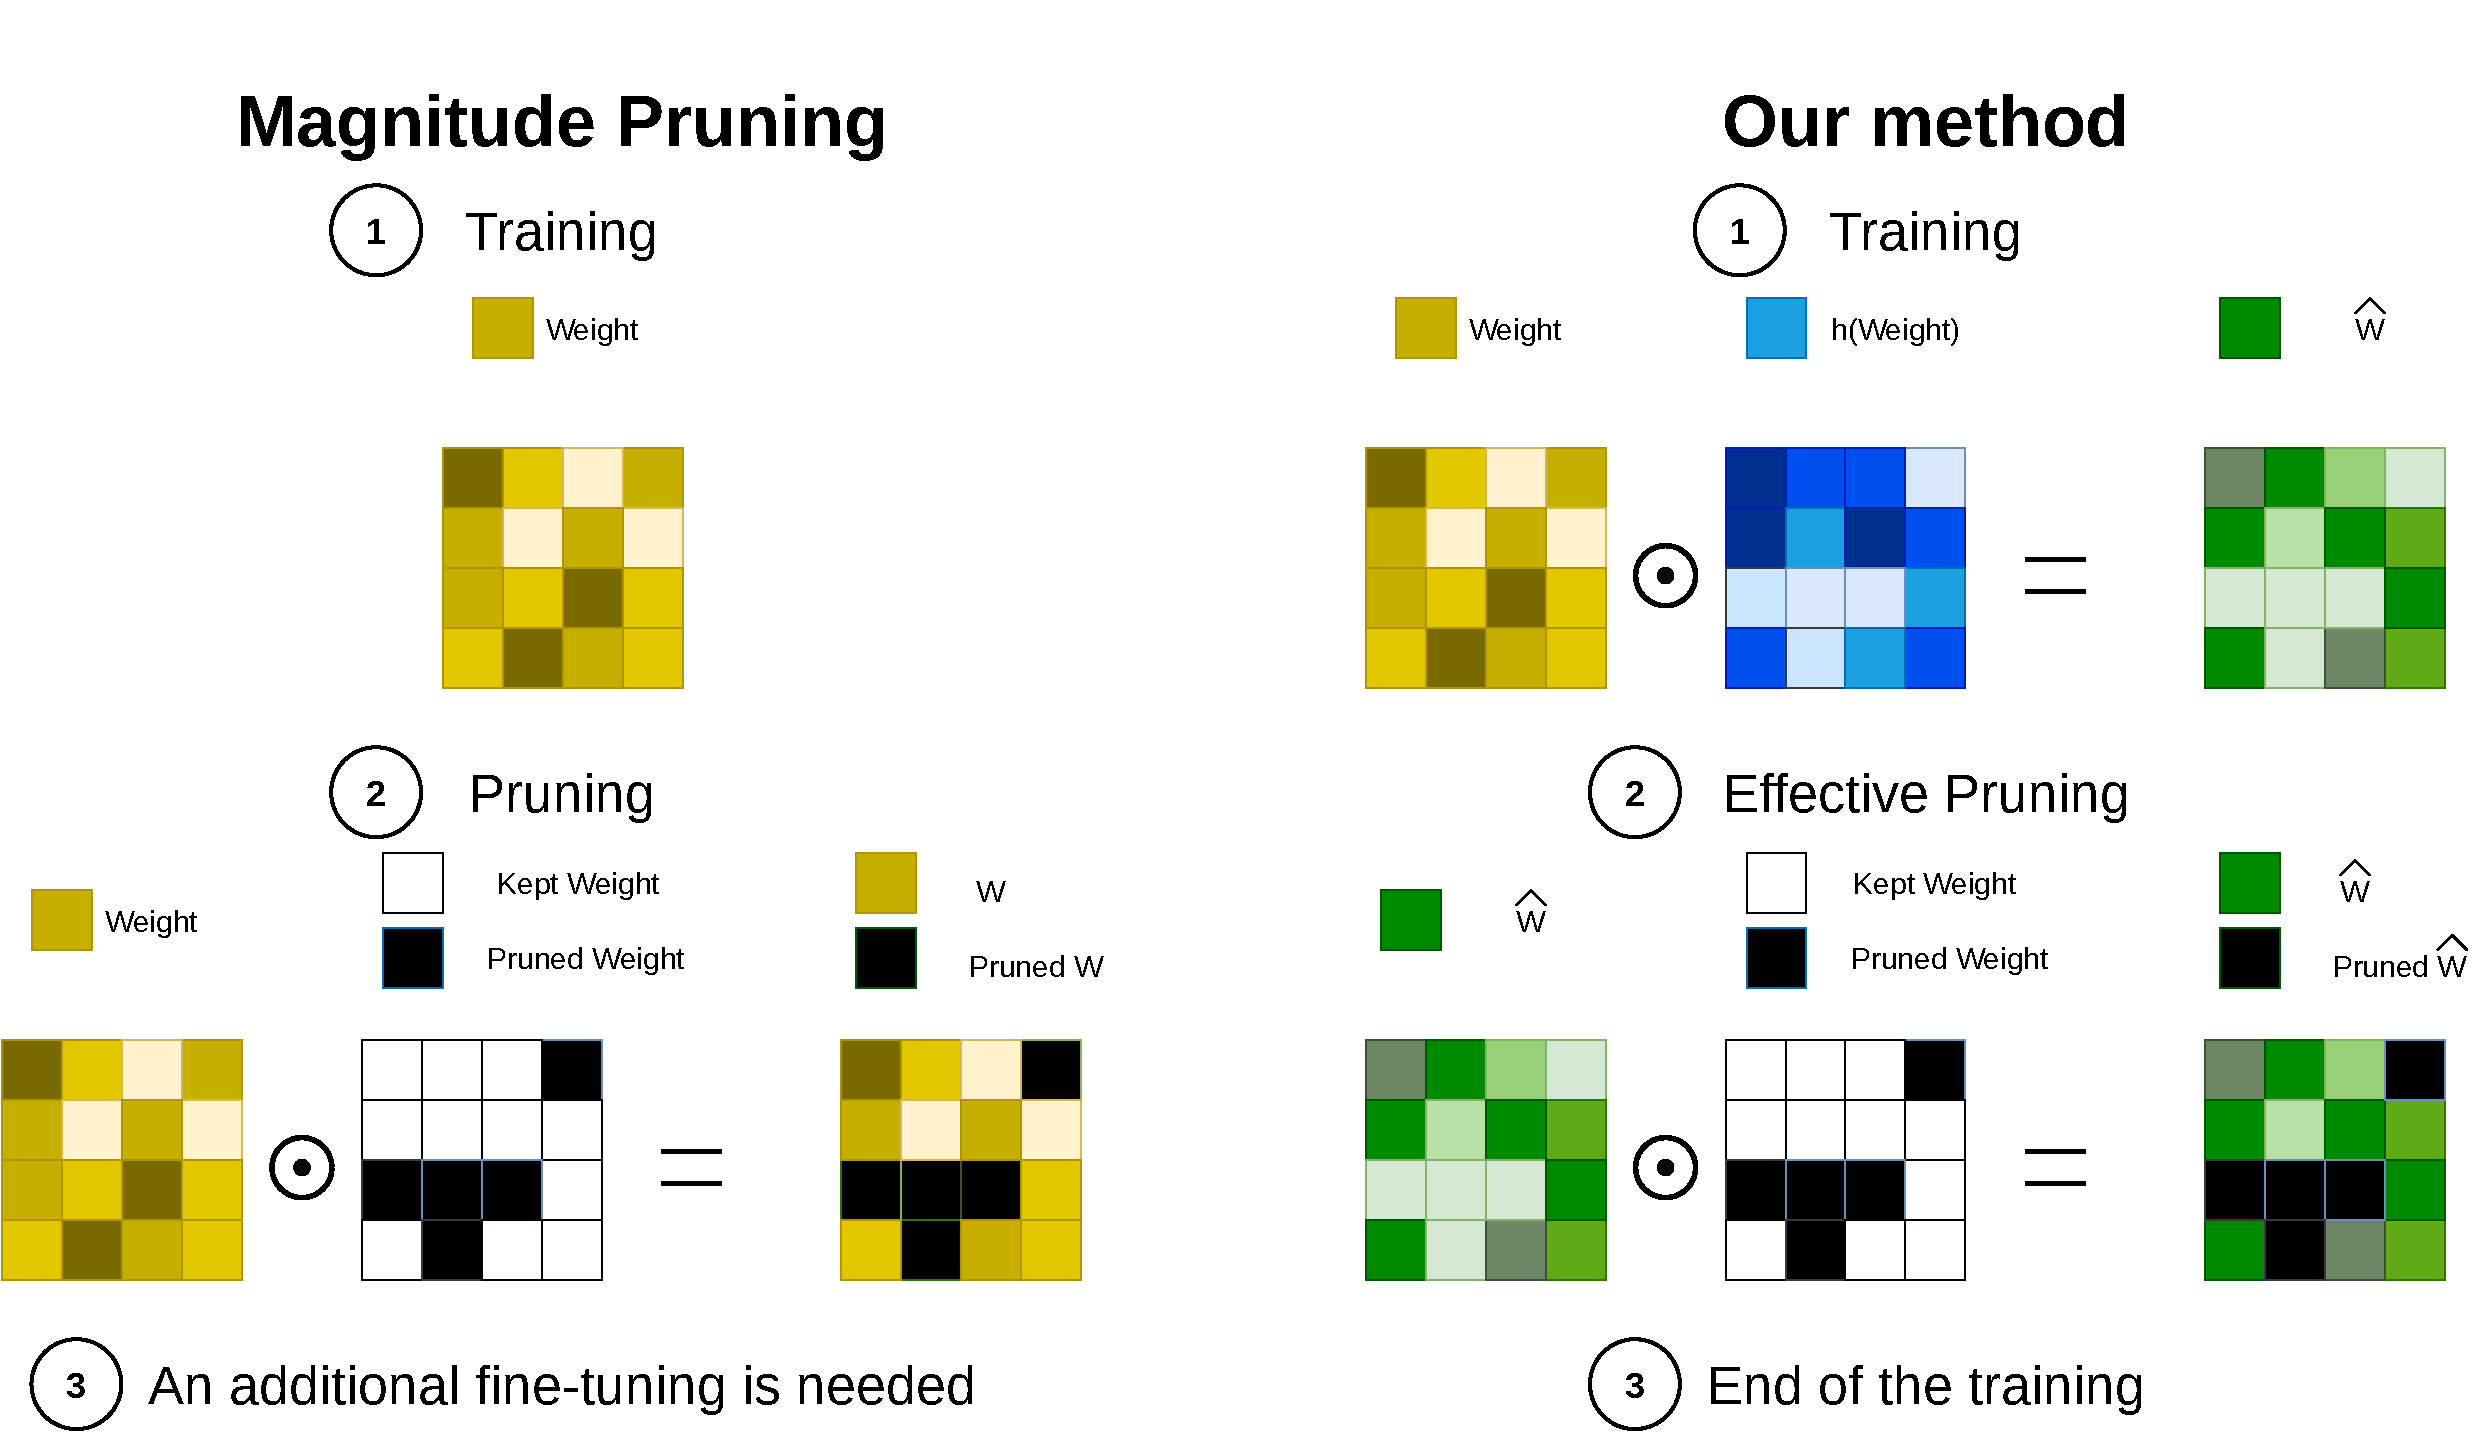
\includegraphics[width=12.5cm]{chapter_1/assets/comparison_reparam_vs_mag_pruning.pdf}}
  \caption{Comparison of our method and magnitude pruning. Magnitude pruning
  does not include any prior on weights during the initial training phase
  and needs an additional fine-tuning procedure. Our method embeds a saliency
  heuristic based on the weight magnitude in the weight reparametrisation and
  does not require fine-tuning.}
  \label{fig:chap1:comparison_reparam_vs_mag_pruning}
\end{figure}


Our proposed framework allows for a joint optimisation of the network weights
and topology. On the one hand, it prevents disconnections which may lead to
degenerate networks with an irrecoverable performance drop. On the other hand,
it allows reaching a targeted pruning budget in a more convenient way than $L_1$
regularisation (cf. \cref{sec:chap1:impact_of_budget_loss}). Our
reparametrisation also helps minimise the discrepancy between the primary and
the surrogate networks by maintaining competitive performances without
fine-tuning. Learning the surrogate network requires only one step that achieves
pruning as a part of network design. This step zeroes out the targeted number of
connections by constraining their reparametrised weights to vanish.

\subsection{Weight Reparametrisation}
\label{sec:chap1:weight_reparam}

We consider the primary network $f$ as a combination of $L$ layers. The global
expression of $f$ can be recursively defined by the application of the layer $\ell$
to the output of the layer $\ell-1$. Without a loss of generality, we omit the
bias for clarity. This expression is shown on
\cref{eqn:chap1:layer_eq_f}.
\begin{equation}
\label{eqn:chap1:layer_eq_f}
f(\mathbf{x}) = g_L \big(\mathbf{w}_L \cdot g_{L-1}(\mathbf{w}_{L-1} \cdot g_{L-2} \dots
\mathbf{w}_2 \cdot g_1(\mathbf{w}_1 \cdot \mathbf{x}))\big),
\end{equation}
\noindent with $g_\ell$ being a nonlinear activation associated to $\ell \in
\left\{ 1,\dots, L \right\}$ and $\left\{ \mathbf{w}_\ell \right\}_\ell$ a
weight tensor. Keeping the same topology but changing the values of the weight,
we now consider the surrogate network $\hat{f}$ with weights
$\{\hat{w}_\ell\}_\ell$. \Cref{eqn:chap1:layer_eq_f} now becomes
\cref{eqn:chap1:layer_eq_f_hat}. The activation function and the topology of $f$
and $\hat{f}$ are the same. Only the weights are changing.

\begin{equation}
\label{eqn:chap1:layer_eq_f_hat}
\hat{f}(\mathbf{x}) = g_L \big(\mathbf{\hat w}_L \cdot g_{L-1}(\mathbf{\hat w}_{L-1} \cdot g_{L-2}
\dots\mathbf{\hat w}_2 \cdot g_1(\mathbf{\hat w}_1 \cdot \mathbf{x}))\big).
\end{equation}

\noindent In the above \cref{eqn:chap1:layer_eq_f_hat}, $\mathbf{\hat w}_\ell$
is referred to as apparent weight. The apparent weight is a reparametrisation of
$\mathbf{w}_\ell$, that includes a prior on its saliency. An apparent weight
$\mathbf{\hat w}_\ell$ of $\hat{f}$ is derived from the standard weight
$\mathbf{w}_\ell$ of $f$ by applying the following reparametrisation: 
\begin{equation}
  \label{eqn:reparam}
  \mathbf{\hat w}_\ell = \mathbf{w}_\ell  \odot h_t(\mathbf{w}_\ell),
\end{equation}
\noindent with $h_t$ being the reparametrisation function and $t$ its
temperature parameter (cf. \cref{eqn:chap1:reparam_prop4}). Here, $\odot$ represents the Hadamar product. It means
that the reparametrisation is element-wise, and every single weight has its own
reparametrisation. This reparametrisation function enforces the prior that
smallest weights should be removed from the network and act as a surrogate $L_0$
norm for the budget loss (see \cref{sec:chap1:budget_loss}). In order to achieve
this objective, $h_t$ should exhibit four properties: \\

\begin{enumerate}
  \item $\forall x \in \mathds{R},~~ 0 \leq h_t(x) \leq 1 $
  \item $h_t(x) \in C^1 \text{ on } \mathds{R}$
  \item $h_t(x) = h_t(-x)$
  \item $\forall a,\varepsilon \in\mathds{R}^{+\ast},~ \exists ~t
  \in\mathds{R}^{+\ast} ~ | ~ h_t(x) \leq \varepsilon, x \in [-a,a]$
\end{enumerate}

\noindent\textbf{First Property - Constrained Image} \\
\begin{equation}
    \centering
    \forall x \in \mathds{R},~~ 0 \leq h_t(x) \leq 1
    \label{eqn:chap1:reparam_prop1}
\end{equation}
\\
There should not be any co-adaptation between the weights and their
reparametrisation. Indeed, the reparametrisation function should not act as a
scaling factor for the weight and scale it so that the apparent weight is larger
than the original weight. Finally, the apparent weight should have the same sign
as the original weight. That is why the image of $\mathbb{R}$ by $h_t$ should be
the segment $[0,1]$.\\

\noindent\textbf{Second Property - Differentiability} \\
\begin{equation}
    \centering
    h_t(x) \in C^1 \text{ on } \mathds{R}
    \label{eqn:chap1:reparam_prop2}
\end{equation}
\\
Our method should fit in the backpropagation method. Since the optimisation will
be achieved by gradient descent, the reparametrisation function should be
derivable to ensure a computable gradient.\\

\noindent\textbf{Third Property - Symmetry} \\

\begin{equation}
    \centering
    h_t(x) = h_t(-x)
    \label{eqn:chap1:reparam_prop3}
\end{equation}
\\
The reparametrisation function should not induce any bias toward the positive or
negative weights so that only their magnitudes matter. It implies that the
reparametrisation function should be symmetric with respect to the origin.\\


\noindent\textbf{Fourth Property - Upper Bounded Segment} \\

\begin{equation}
    \centering
    \forall a,\varepsilon \in\mathds{R}^{+\ast},~ \exists ~t
    \in\mathds{R}^{+\ast} ~ | ~ h_t(x) \leq \varepsilon, x \in [-a,a]
    \label{eqn:chap1:reparam_prop4}
\end{equation}
\\
The last property ensures the existence of a temperature parameter $t$, which
allows upper-bounding the response of $h_t$ on any interval for any arbitrary
$\varepsilon$. More formally, for any arbitrarily large $a$ and arbitrarily
small $\varepsilon$, it exists a temperature $t$ which guarantees that the
reparametrisation of any $x$ is smaller than $\varepsilon$, provided that $x$ is
in the segment $[-a, a]$. Hence, $h_t$ acts as a stopband filter, eliminating
the smallest weights where the parameter $t$ controls the width of that filter.
\Cref{fig:chap1:reparam_funct_varying_t} shows the impact of $t$ on the shape of
the function, more precisely on the width of its pit, when the expresion of
$h_t$ is the one of \cref{eqn:chap1:stable_h_expression}.\\

\begin{figure}
    \centering
    \subfloat[$h_{t}$ with $t=1$ and varying $n$]{
        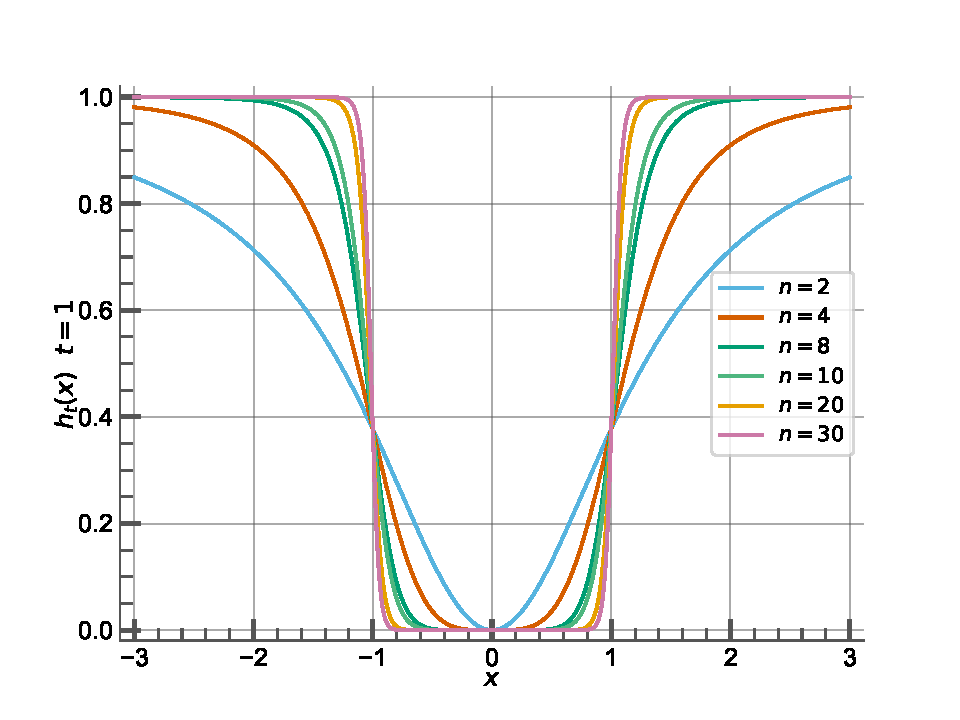
\includegraphics[width=0.49\linewidth]{chapter_1/assets/reparam_funct_varying_n.pdf}
        \label{fig:chap1:reparam_funct_varying_n}} \subfloat[$h_{t}$ with $n=2$
    and varying $t$]{
        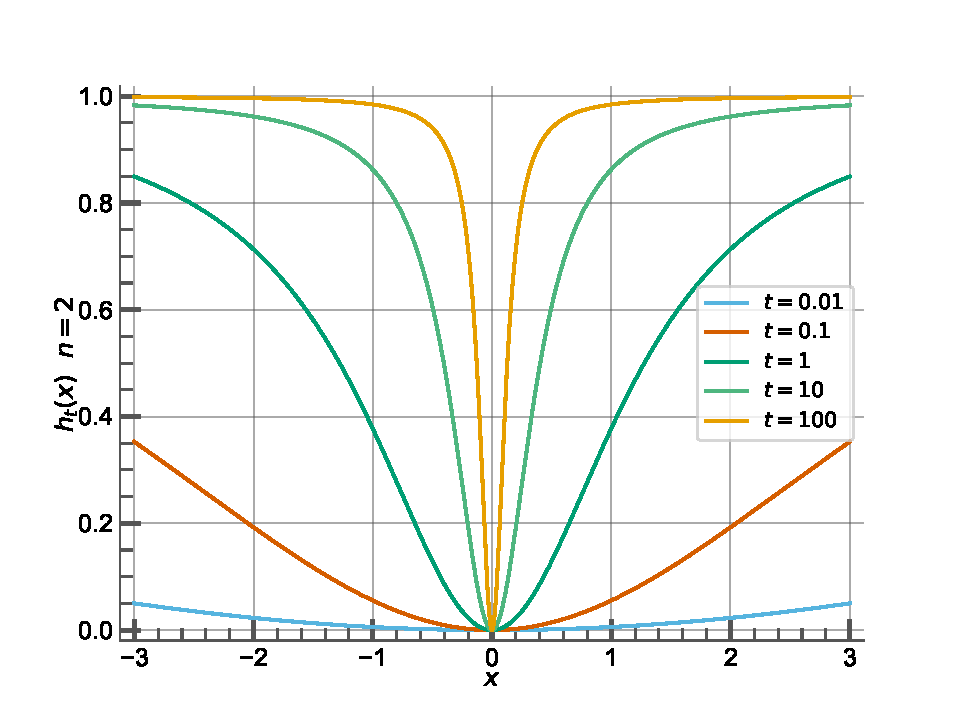
\includegraphics[width=0.49\linewidth]{chapter_1/assets/reparam_funct_varying_t.pdf}
        \label{fig:chap1:reparam_funct_varying_t}} \caption{
    Reparametrisation function $h_t$ with varying temperature parameter $t$ and
    power $n$. $t$ controls the width of the pit, and $n$ controls the steepness
    of the slope.}
    \label{fig:stopband}
\end{figure}

Weight distribution varies tremendously from one layer to another. In order to
match a specific budget (cf. \cref{sec:chap1:budget_loss}), the width of the
stopband, controlled by $t$, is tuned according to the weight distribution of
each layer. The manual setting of this parameter is non-trivial and cumbersome,
so in practice, $t$ is learned as a part of gradient descent on a layer-by-layer
basis.\\

% TODO: Ajouter amorce pour discussions sur l'initialisation de la température.
%the initial setting  $t_\text{init}$ of this temperature is shown in
%\cref{tbl:pruningperformances}.\\


Considering the aforementioned four properties of $h_t$, a simple choice of that
function is:
\begin{equation}
  \label{eqn:chap1:h_star_expression}
  h_t^*(x) = \exp\bigg\{{-\displaystyle\frac{1}{(tx)^n}}\bigg\}, ~ n\in 2\mathds{N},
\end{equation}
\noindent where $n$ controls the crispness of $h_t^*$. $n$ is not considered as
a parameter of $h_t$ (or $h_t^*$) since we use a fixed value for our
experiments, whereas $t$ is a learnt parameter and varies from one layer to
another. \Cref{fig:chap1:reparam_funct_varying_n} show the impact of n on the
general sharpness of the function. Although the function described in
\cref{eqn:chap1:h_star_expression} satisfies the four above properties, $h_t^*$
suffers from numerical instability as it generates \ac{nan} outputs in most of
the widely used deep learning frameworks. Due to the way Backpropagation works,
a single \ac{nan} in a weight tensor makes the whole optimisation process for
the entire network no longer possible. We consider instead a stabilised variant
with similar behaviour, as \cref{eqn:chap1:h_star_expression},  that still
satisfies the four above properties. This numerically stable variant is defined
as:
\begin{equation}
  \label{eqn:chap1:stable_h_expression}
  h_t(x) = C_1 \biggl( \text{exp} \bigg\{-\displaystyle\frac{1}{(tx)^n +1}\bigg\} - C_2 \biggr),
\end{equation}
\noindent with $C_1=\frac{1}{1-e^{-1}}$ and $C_2 = e^{-1}$.\\

The addition of the scalar value 1 at the denominator in
\cref{eqn:chap1:stable_h_expression} is a mean to achieve numerical stability.
In equation \cref{eqn:chap1:h_star_expression}, the denominator $(tx)^n$ has the
potential to approach very small values that result in numerical instabilities,
leading to \ac{nan} outputs. The addition of 1 to the denominator makes the
function numerically stable and avoids producing \ac{nan} outputs. This solution
is favoured over adding a small value, such as an arbitrarily small
$\varepsilon$, as the latter requires careful consideration of its magnitude and
may result in either dramatic alterations to the shape of the function or
continued numerical instability if not carefully chosen. The addition of the
value 1 to the denominator provides a straightforward and sufficient mean to
stabilise the function. Constants $C_1$ and $C_2$ are introduced to compensate
for the slight alterations to the shape of the function caused by the addition
of 1 to the denominator, and thus, to ensure that the first property
(\cref{eqn:chap1:reparam_prop1}) is respected. Although both $h_t^*$ and $h_t$
satisfy the four properties, they do not possess the exact same shapes, as
demonstrated in figure (\ref{fig:chap1:h_stable_vs_unstable}).\\

\begin{figure}
  \centering
  \centerline{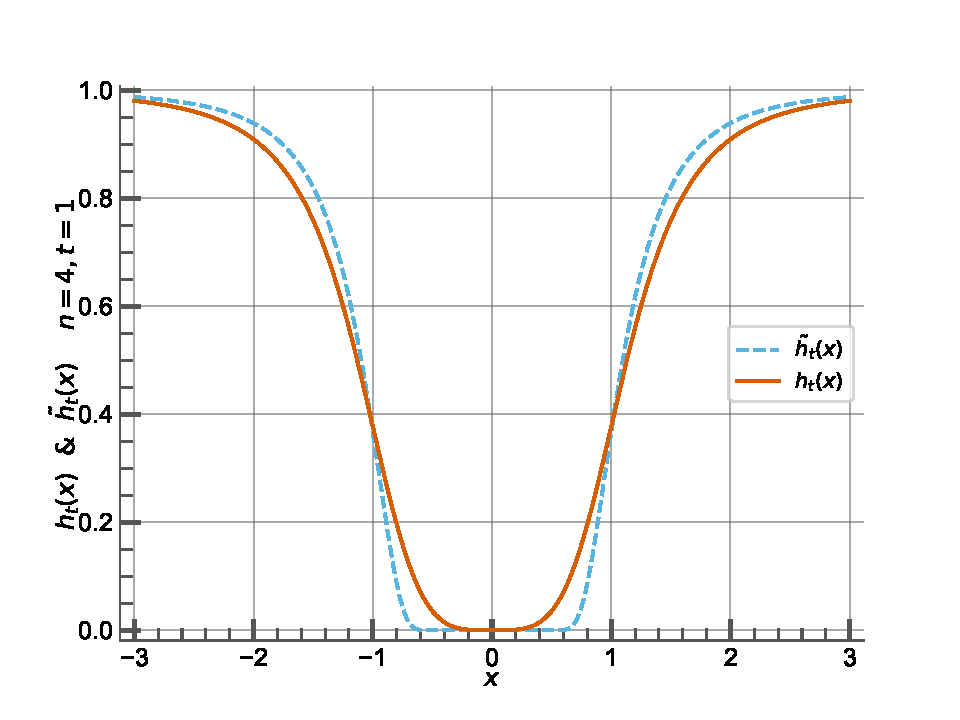
\includegraphics[width=0.49\linewidth]{chapter_1/assets/h_stable_vs_unstable.pdf}}
  \caption{ The unstable reparametrisation function $h_t^*$ and its
  stable alternative $h_t$, with $t=1$ and $n=4$ for both functions.} 
  \label{fig:chap1:h_stable_vs_unstable}
\end{figure}

\subsection{Budget Loss}
\label{sec:chap1:budget_loss}

Most traditional pruning methods in deep learning do not explicitly incorporate
the target weight budget during the optimisation procedure. The amount of
weights pruned is typically enforced post-training, which can lead to suboptimal
results compared to methods that consider the weight budget during optimisation.
Our method introduces a budget loss term, in addition to the main task loss
term, that drives the network to match and respect a given weight budget during
the training process. Consequently, the trained network can be pruned to the
desired pruning rate with a marginal loss in performance and does not need
fine-tuning.\\


The considered budget is weight-based and should quantify the target fraction of
active connections in the network. To build the budget loss, we first introduce
a cost function that quantifies the number of active connections in the network.
Let $C(\{\mathbf{w}_1,\dots, \mathbf{w}_L\})$ be the {\em current} cost
associated to a neural network and its set of {\em current} weights and
$C_\text{target}$ the {\em targeted} one. $C_\text{target}$ is the number of
connections that should be active at the end of the training procedure. The
budget loss is defined as \\

\begin{equation}
  \label{eqn:chap1:simple_budget}
  {\cal L}_\text{budget} = \bigl( C(\{\mathbf{w}_1,\dots, \mathbf{w}_L\}) - C_\text{target} \bigr)^2.
\end{equation} \\


\noindent This budget loss is combined with the main task loss (a classification
loss in our experiments - see \cref{sec:chap1:experiments}). The budget loss $
{\cal L}_\text{budget}$ is in quadratic form to ensure the minimisation of this
loss will, in turn, minimise the difference between the {\em current} cost and
the {\em targeted} one. For better conditioning of this combination, we
normalise the budget loss by $C_\text{initial}$. The latter corresponds to the
cost of the primary unpruned network, which is set in practice to the number of
its parameters (see also \cref{sec:chap1:experiments}). Hence,
\cref{eqn:chap1:simple_budget} is updated as:\\

\begin{equation}
  \label{eqn:chap1:real_budget}
  {\cal L}_\text{budget} = \biggl( \displaystyle\frac{C(\{\mathbf{w}_1,\dots, \mathbf{w}_L\}) - C_\text{target}}{C_\text{initial}} \biggr)^2.
\end{equation}\\

Finally, the two losses are combined together via a strictly positive mixing
parameter $\lambda$ that  controls the relative importance of  the budget loss
${\cal L}_\text{budget}$ compared to the main task loss ${\cal L}_\text{task}$,
leading to\\

\begin{equation}
  \label{eqn:chap1:globalloss}
   {\cal L} =  {\cal L}_\text{task} + \lambda \cdot {\cal L}_\text{budget}.
\end{equation} \\

Ideally, the budget of a neural network could be evaluated as the number of
multiply-add operations, often referred to as \ac{FLOPs}, needed for a forward
pass or through the $L_0$ norm of its weights. However, neither are known to
be differentiable and, therefore, cannot be used in a gradient-based
optimisation. In order to circumvent these limitations, we use our weight
reparametrisation as a surrogate measure of $L_0$, and we define the cost
function as \\

\begin{equation}
  \label{eqn:chap1:cost_function}
  C(\{\mathbf{w}_1,\dots, \mathbf{w}_L\}) = \displaystyle \sum_{i=1}^{L} h_t(\mathbf{w}_i). 
\end{equation} \\


\begin{figure}
  \centering
  \subfloat[Number of parameters]{
      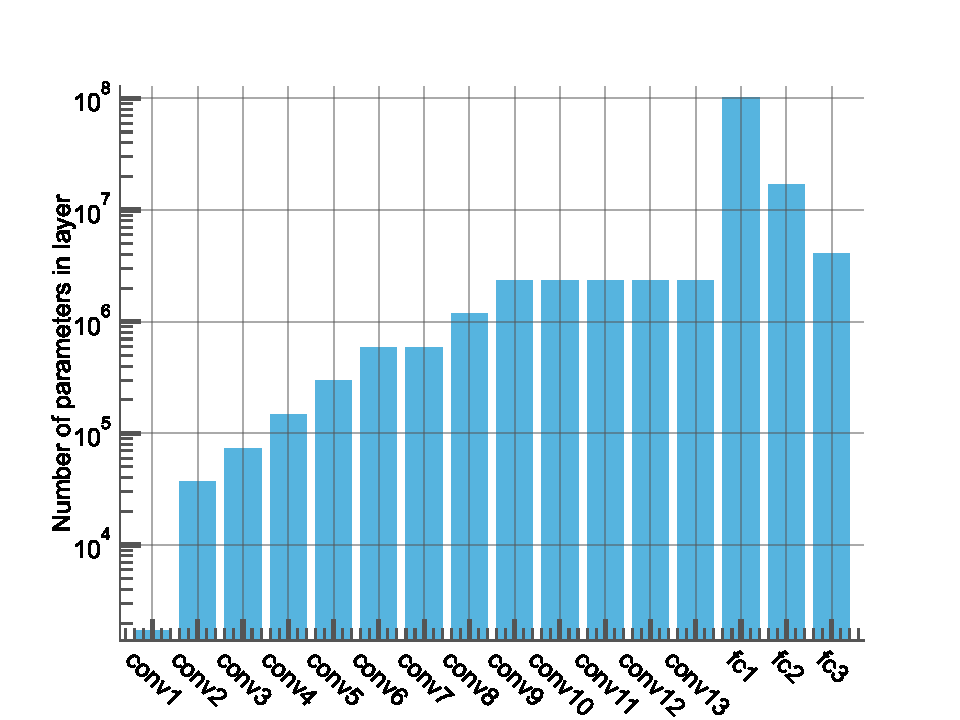
\includegraphics[width=0.49\linewidth]{chapter_1/assets/vgg16_num_params_per_layer.pdf}
      \label{fig:chap1:num_parap_vgg16}} \subfloat[Normalisation factor]{
      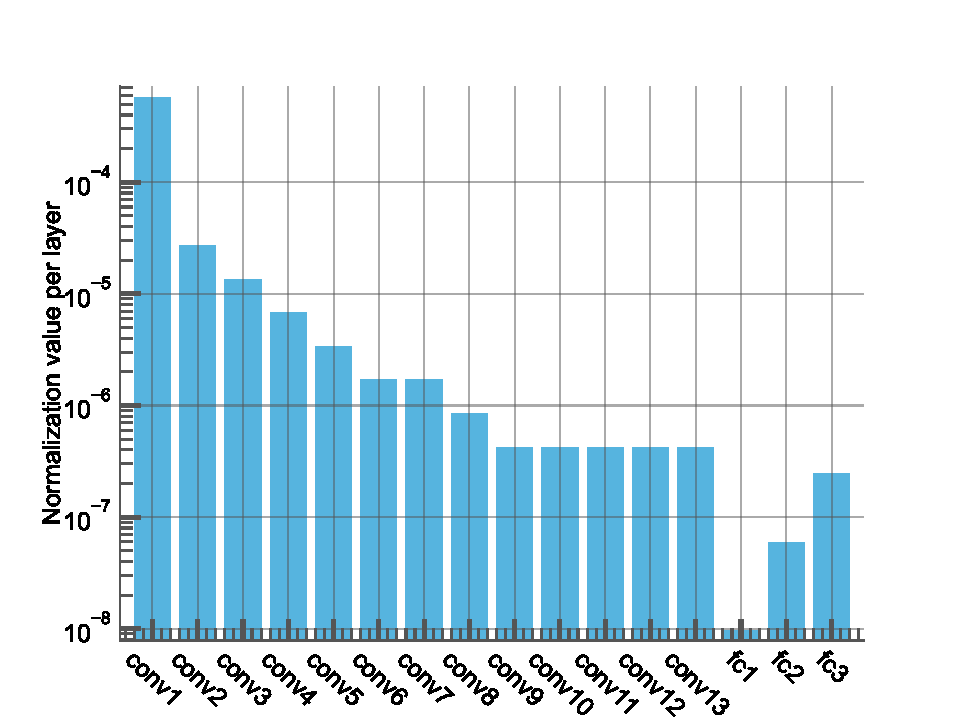
\includegraphics[width=0.49\linewidth]{chapter_1/assets/vgg16_normalization_factor_per_layer.pdf}
      \label{fig:chap1:norm_factor_vgg16}} \caption{ Log-scale plot of
      number of parameters and normalisation factor per layer for a VGG16
      network. The significant differences in terms of the number of parameters
      yields dramatically different normalisation factors. Some of them are 4
      orders of magnitude apart, and all of them are vanishingly small compared
      to a common main task loss value.} 
  \label{fig:chap1:vgg16_per_layer_param_and_norm_factor}
\end{figure}

One could argue that the cost should be normalised layer-wise and, therefore,
that the right-hand term of \cref{eqn:chap1:cost_function} should be written as
$$\displaystyle\sum_{i=1}^{L}\frac{h_t(\mathbf{w}_i)}{\text{Card}(\mathbf{w}_i)}$$
where $\text{Card}(.)$ denotes the cardinal function, it is to say, in this
case, the number of scalar elements in a weight tensor. However, the number of
elements in a layer greatly varies from one layer to another (as demonstrated in
\cref{fig:chap1:vgg16_per_layer_param_and_norm_factor}). As a result,  the
budget loss relative importance would vary from one layer to another. More
importantly, the optimisation process would have less incentive to introduce
sparsity in larger layers since their normalisation factor would make the budget
loss negligible compared to other layers or the main task loss. This is critical
since the large layers are generally the ones where the highest pruning rates
can be achieved \cite{DBLP:journals/corr/abs-2202-12002}. Regarding the
aforementioned reasons, a better alternative is to normalise by the initial cost
$C_\text{initial}$, as done in \cref{eqn:chap1:real_budget}.\\

% endregion

\section{Overview}
\label{sec:chap1:overview}

Our method is a combination of a weight reparametrisation and a budget loss. The
two are combined in a global method that can be used in a standard training
procedure using gradient descent. In the \cref{sec:chap1:experiments} our
results are obtained after following the procedure described in
\cref{alg:chap1:training_pruning}. In \cref{sec:chap1:impact_of_fine_tuning} the
procedure is the same, except that the \emph{effective pruning} is applied before the
training, which in this case is called fine-tuning because the initial weights
$\theta$ are already tuned.\\

\begin{algorithm}
  \caption{Our training procedure}
  \label{alg:chap1:training_pruning}
  \begin{algorithmic}
  \REQUIRE Dataset $\mathcal{D} = \{\mathcal{X}, \mathcal{Y}\}$, network $f$,
  weights $\theta$, number of epochs $n$, mixing coefficient $\lambda$, learning
  rate $\eta$, pruning rate $p$
  \FOR{$t = 1$ to $n$}
      \FOR{each $(x,y) \in \mathcal{D}$}
          \STATE Compute the output of the network $\hat{y} = f(x; \theta_t)$
          \STATE Compute the loss $\mathcal{L}= \mathcal{L}_{task}(y, \hat{y}) + \lambda \cdot \mathcal{L}^{p}_{budget}(\theta_t)$
          \STATE Backpropagate the loss and update the weights $\theta_{t+1} = \theta_t - \eta \nabla_{\theta} \mathcal{L}$
      \ENDFOR
  \ENDFOR
  \RETURN Trained network $f$
  \STATE Perform \emph{effective pruning} on the weights $\theta$: set to 0 the
  smallest $p$\% of the weights $w\in\theta$
  \RETURN Trained and pruned network $f$
  \end{algorithmic}
  \end{algorithm}


The interested reader can grasp a better understanding of the key differences of
our method compared to the standard pruning pipeline that applies to most
pruning methods, not only magnitude pruning method, by looking at
\cref{fig:chap1:pruning_pipeline_comparison}. It highlights the fact that the
target pruning rate is taken into account from the beginning thanks to the budget
loss, and therefore, the network does not need a fine-tuning step after the
\emph{effective pruning} step. On the contrary, the standard pruning pipeline
applies the \emph{pruning criterion} and the \emph{effective pruning} after the
initial training. This results in a drop in performance that needs to be
compensated for with fine-tuning. \\

\begin{figure}
\centering
\subfloat[Our Pipeline\label{fig:chjap1:our_pipeline}]{
  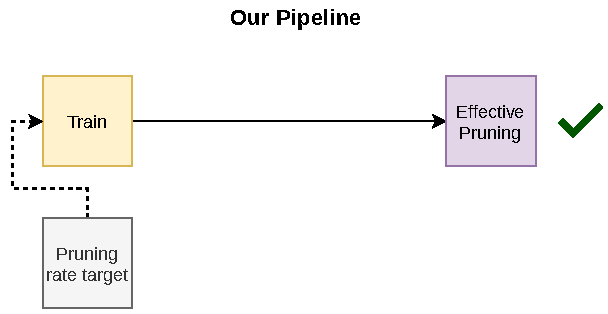
\includegraphics[width=0.49\textwidth]{chapter_1/assets/pipeline_comparison_with_pruning_reparam_pr.pdf}}
\subfloat[Standard Pruning Pipeline\label{fig:chap1:standard_pruning_pipeline}]{
  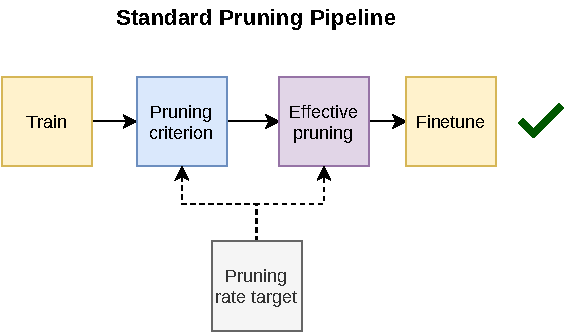
\includegraphics[width=0.49\textwidth]{chapter_1/assets/pipeline_comparison_with_pruning_mag_pr.pdf}}
  \caption{ Principle scheme of our pruning pipeline and the standard
  pruning pipeline. With our pruning pipeline, the target pruning rate that will
  be enforced during the \emph{effective pruning} step, is taken into account
  from the beginning. Thus, our method does not need a fine-tuning step. In
  contrary, the standard pruning pipeline applies the \emph{pruing criterion}
  and the \emph{effective pruning} after the initial training. This results in a
  drop in performance that needs to be compensated for with fine-tuning.}
  \label{fig:chap1:pruning_pipeline_comparison}
\end{figure}

\section{Experiments And Results}
\label{sec:chap1:experiments}

In this section, we will explore the effectiveness of our method on deep neural
networks for image classification. We have chosen to use three reference
databases in the field of computer vision: CIFAR10 \cite{CIFARdataset}, CIFAR100
\cite{CIFARdataset}, and TinyImageNet \cite{TinyImageNet}. We will evaluate the
impact of our method on several neural network architectures: VGG16
\cite{DBLP:journals/corr/SimonyanZ14a}, Conv4 \cite{DBLP:conf/iclr/FrankleC19},
ResNet18, and ResNet20 \cite{DBLP:conf/cvpr/HeZRS16}. This study will allow us
to demonstrate the effectiveness of our method for compressing image
classification models, as well as its influence on the performance, which is the
prediction accuracy in this case. To that extent, we will review the impact of
both our reparametrisation and our budget loss.\\

The CIFAR10 and CIFAR100 datasets both contain 60,000 colour images of size
32x32 pixels, split into 10 and 100 classes, respectively. The TinyImageNet
dataset is shrunk version of the ImageNet dataset
\cite{DBLP:journals/ijcv/RussakovskyDSKS15}, and contains 100,000 images of size
64x64 pixels, split into 200 classes. Each dataset is divided into two folds: a
training set and a test set. In addition to these two folds, we also use a
validation set to tune the hyperparameters of our method before testing it on
the test set. The validation dataset is obtained by selecting 10\% of the
training set. \Cref{tab:chap1:datasets} summaries the composition of the three
datasets.\\


\begin{table}[ht]
  \centering
  \begin{tabular}{lcccc}
    \toprule
    \textbf{Dataset} & \textbf{Number of images} & \textbf{Number of classes} &
    \textbf{Image size} & \textbf{Size of test set} \\ 
    \hline
    CIFAR10 & 60,000 & 10 & 32x32 & 10,000 \\ 
    CIFAR100 & 60,000 & 100 & 32x32 & 10,000\\ 
    TinyImageNet & 100,000 & 200 & 64x64 &10,000 \\ 
    \bottomrule
  \end{tabular}
  \caption{The number of images, of classes, image size and size of the test set for the three datasets used.}
  \label{tab:chap1:datasets}
\end{table}

In combination with these datasets, we use four different neural networks. Conv4
is a small and reasonably lightweight convolutional neural network which is a
shrunk-down version of the VGG16 architecture. VGG16 is a convolutional neural
of larger size and depth, which is a popular choice for image classification. We
used a slightly modified version of VGG16 that is better suited to CIFAR10. We
do not use dropout, but we use batch normalisation, and the fully connected
section has only one layer. ResNet18 is a residual neural network that
introduces skip connection in its architectural design. ResNet20 is a modified
version of the ResNet18 architecture to make it suited for CIFAR10 and CIFAR100
datasets. \Cref{tab:chap1:networks_size} summarises the size of the different
models. In our experiments, we use ResNet18 exclusively for TinyImageNet and the
other networks for CIFAR10 and CIFAR100.\\


\begin{table}[ht]
  \centering
  \begin{tabular}{lcccc}
  \cline{2-5}
                       & \textbf{Conv4}     & \textbf{VGG16}      & \textbf{ResNet20} & \textbf{ResNet18}   \\ \hline
  Number of Parameters & 2,425,930 & 14,728,266 & 269,034  & 11,685,608 \\ \hline
  \end{tabular}
  \caption{ number of parameters for the four neural network architectures used.}
  \label{tab:chap1:networks_size}
\end{table}

\subsection{Performances}
\label{sec:chap1:performances}
Performances of our method are evaluated on CIFAR10 and CIFAR100 with Conv4,
VGG16 and ResNet20. On TinyImageNet, we evaluate our method on ResNet18. We
compare our method against magnitude pruning \cite{DBLP:conf/nips/HanPTD15}. The
key differences between our method and magnitude pruning are the following:
$(i)$ our method uses a budget loss to encourage sparsity, which takes into
account the final pruning rate from the beginning of the training process,
$(ii)$ our method does not require fine-tuning after pruning. Because of the
latter, we compare our method against magnitude pruning with and without
fine-tuning. Both methods share the following setup: networks are trained during
300 epochs with an initial learning rate of 0.1. A {\em Reduce On Plateau}
policy is applied to the learning rate: if the validation accuracy is not
improving for 10 epochs in a row, then the learning rate is decreased by a
factor of 0.3. A weight decay is applied on the weights with a penalisation
factor of $5\times10^{−5}$. This value is lower than the more conventional value
of $1\times10^{-4}$, because we want some weights to be able to drift away from the
origin, and therefore, escape from the pit of $h_t$. An Early Stopping policy was
used to stop the training prematurely if no improvement of the test accuracy is
observed in 60 epochs. To keep the comparison fair, for magnitude pruning, the
300 epochs are split into two phases: the first 150 epochs are dedicated to the
training of the network, and the last 150 epochs are used for fine-tuning the
pruned network. In the fine-tuning phase, the learning rate is divided by 100
for better convergence. \\

Results are repported on
\cref{fig:chap1:reparam_vs_mpft_conv4,fig:chap1:reparam_vs_mpft_resnet20,fig:chap1:reparam_vs_mpft_vgg16}.
In the figures mentioned above, our method (denoted \emph{Ours}) is compared to
magnitude pruning with and without fine-tuning (denoted \emph{MP w/ FT} and
\emph{MP w/o FT}, respectively). All three methods are evaluated on the test
fold of the dataset once the network has been pruned up to the pruning rate
indicated on the \emph{x-axis}. The test accuracy is reported on the \emph{y-axis} as a float between
0 and 1 (0 being all images wrongly classified and 1 being all images correctly
classified). Each solid line representing a method is the mean of 5 independent
runs. The coloured area surrounding the solid line represents the range within
plus or minus one standard deviation. In addition to the three methods, the
dashed lines represent the performances of an unpruned network trained without
weight reparametrisation and budget loss (denoted \emph{baseline}) and the
accuracy of our method before the effective pruning (denoted \emph{Ours (pre
pruning)}). Sub-figures (c) and (d) of
\cref{fig:chap1:reparam_vs_mpft_conv4,fig:chap1:reparam_vs_mpft_resnet20,fig:chap1:reparam_vs_mpft_vgg16}.
represents the number of epochs (\emph{y-axis}) needed to obtain the best model
for each method, depending on the pruning rate (\emph{x-axis}).\\


Overall, our method performs consistently better than magnitude pruning without
fine-tuning (\emph{MP w/o FT}) and, for almost all pruning rates, better than
magnitude pruning with fine-tuning (\emph{MP w/ FT}) on the CIFAR10 and CIFAR100
datasets. In particular, our method significantly outperforms magnitude pruning
in both setups (with and without fine-tuning) for Conv4 networks (cf.
\cref{fig:chap1:reparam_vs_mpft_conv4_cifar10}). For the VGG16 network, we
observe the same trend, although the difference is less significant. For
ResNet20, magnitude pruning slightly overperforms our method on CIFAR100 for
high pruning rates (more than 90\%).
\Cref{fig:chap1:reparam_vs_mpft_conv4_cifar10_epochs,fig:chap1:reparam_vs_mpft_conv4_cifar100_epochs,fig:chap1:reparam_vs_mpft_vgg16_cifar10_epochs,fig:chap1:reparam_vs_mpft_vgg16_cifar100_epochs,fig:chap1:reparam_vs_mpft_resnet20_cifar10_epochs,fig:chap1:reparam_vs_mpft_resnet20_cifar100_epochs}
show that our method requires an equivalent number of epochs compared to
magnitude pruning for a higher level of performance (i.e. a higher test
accuracy). Magnitude pruning requires fewer epochs than our method, only at high
pruning rates (more than 90\%). On TinyImageNet
(\cref{fig:chap1:reparam_vs_mpft_resnet18}), our method outperforms magnitude
pruning with and without fine-tuning up until very high pruning rates (95\%). In
any cases
(\cref{fig:chap1:reparam_vs_mpft_conv4,fig:chap1:reparam_vs_mpft_vgg16,fig:chap1:reparam_vs_mpft_resnet20,fig:chap1:reparam_vs_mpft_resnet18}),
Our method produces much more stable results, and variations from one run to
another are significantly slimmer than the ones in magnitude pruning. Indeed,
the combination of the reparametrisation and the budget loss act, on the one
hand, as a regulariser and, on the other hand, helps to prepare the network for
the effective pruning step.\\

% region: perfs_figures
\begin{figure}
  \centering
  \subfloat[Conv4 - CIFAR10]{
      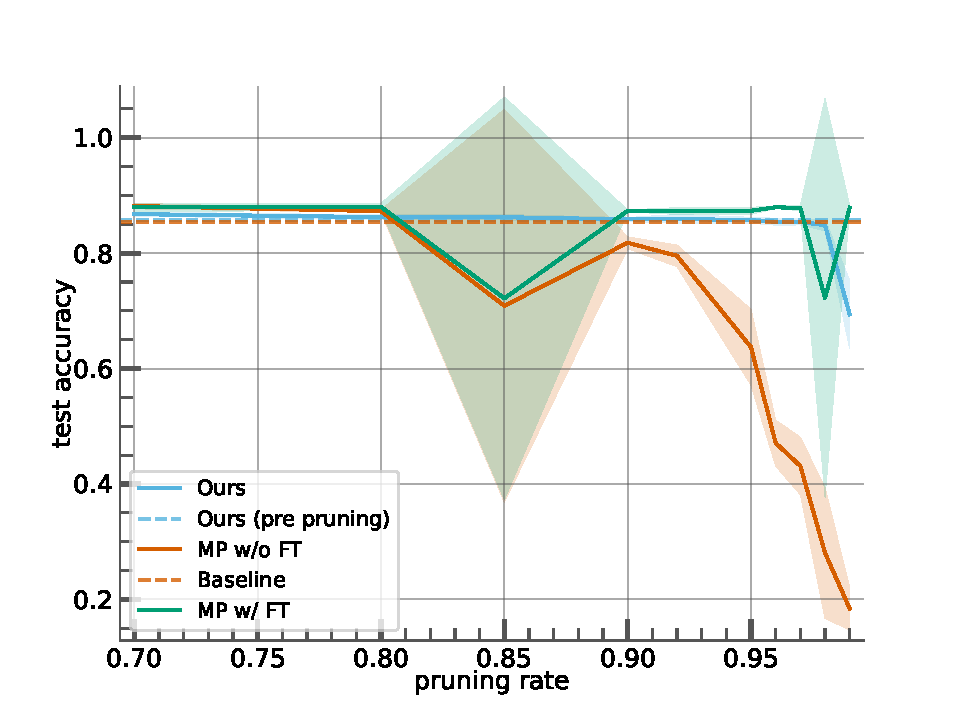
\includegraphics[width=0.49\linewidth]{chapter_1/assets/reparam_vs_mpft_Conv4_cifar10.pdf}
      \label{fig:chap1:reparam_vs_mpft_conv4_cifar10}}
  \subfloat[Conv4 - CIFAR100]{
      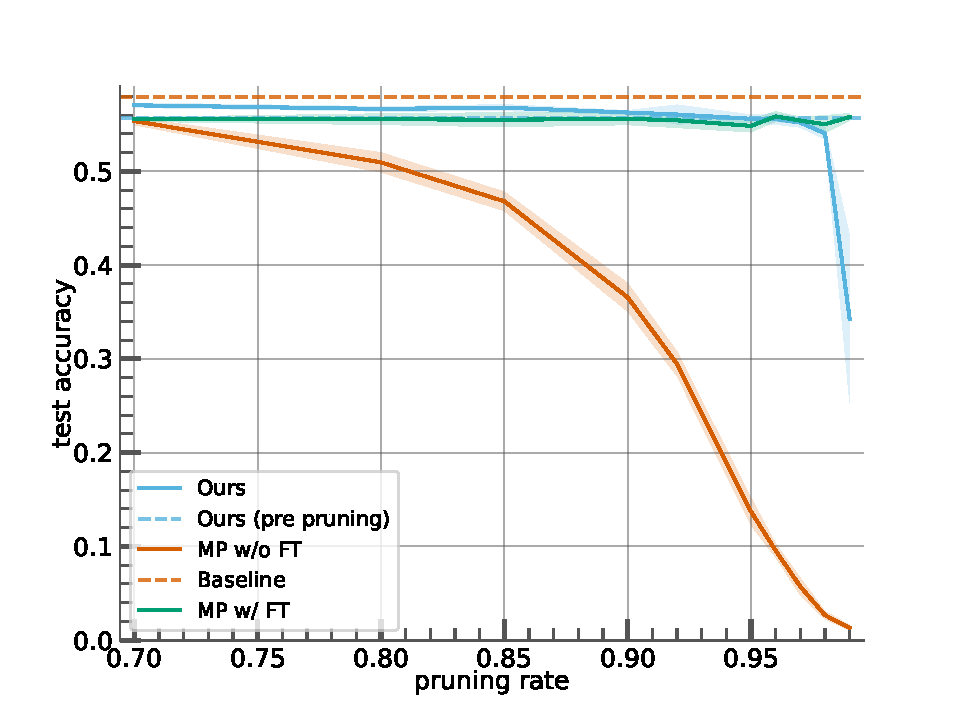
\includegraphics[width=0.49\linewidth]{chapter_1/assets/reparam_vs_mpft_Conv4_cifar100.pdf}
      \label{fig:chap1:reparam_vs_mpft_conv4_cifar100}}
      \\
  \subfloat[Conv4 - CIFAR10 (Number of Epochs)\label{fig:chap1:reparam_vs_mpft_conv4_cifar10_epochs}]{
      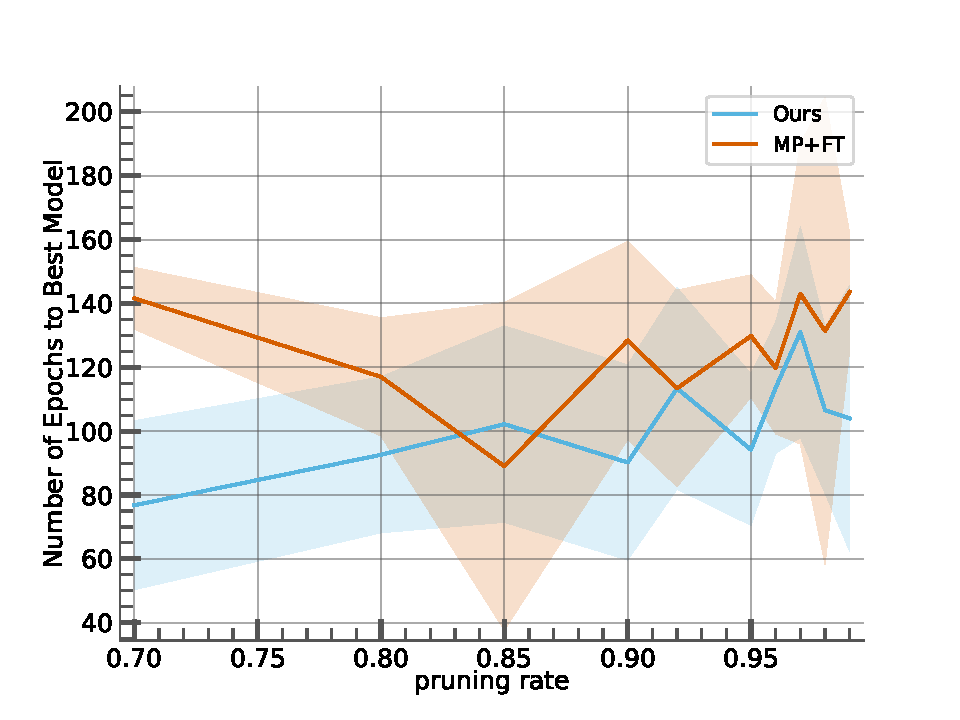
\includegraphics[width=0.49\linewidth]{chapter_1/assets/reparam_vs_mpft_training_time_Conv4_cifar10.pdf}}
  \subfloat[Conv4 - CIFAR100 (Number of Epochs)\label{fig:chap1:reparam_vs_mpft_conv4_cifar100_epochs}]{
      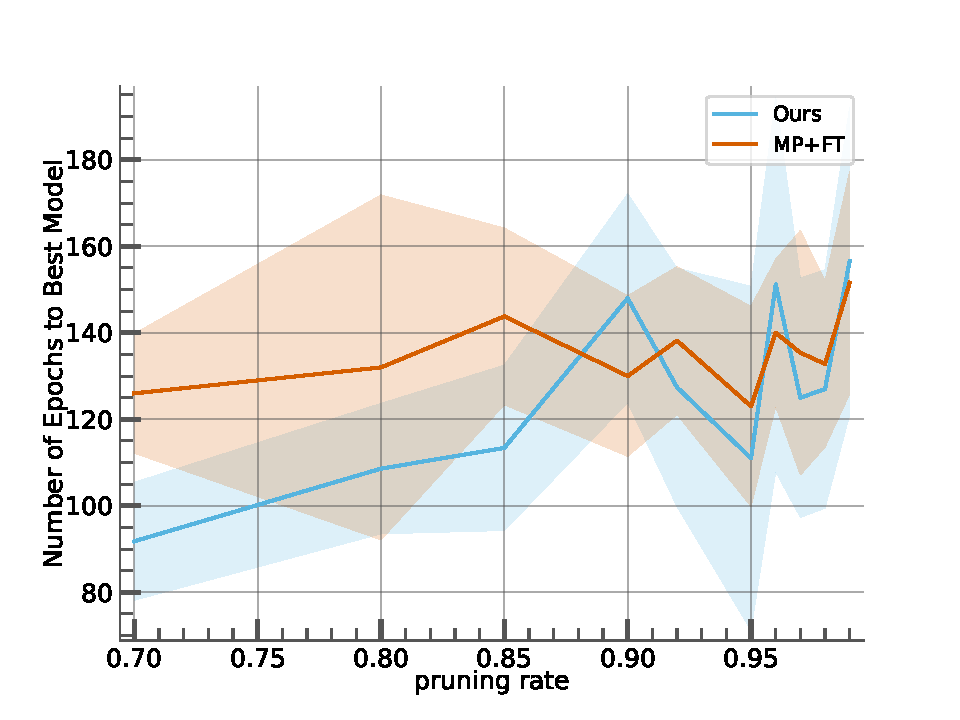
\includegraphics[width=0.49\linewidth]{chapter_1/assets/reparam_vs_mpft_training_time_Conv4_cifar100.pdf}}
  \caption{ Performances comparison of our method {\em(Ours)} against
  magnitude pruning without {\em(MP w/o FT)} and with fine-tuning {\em(MP w/ FT)} with a Conv4 network on
  CIFAR10 and CIFAR100 datasets, for different pruning rates.
  \Cref{fig:chap1:reparam_vs_mpft_conv4_cifar10} and
  \cref{fig:chap1:reparam_vs_mpft_conv4_cifar100} show the testing accuracy of
  the model and \cref{fig:chap1:reparam_vs_mpft_conv4_cifar10_epochs} and
  \cref{fig:chap1:reparam_vs_mpft_conv4_cifar100_epochs} the number of epochs
  needed to obtain the best model.}
  \label{fig:chap1:reparam_vs_mpft_conv4}
\end{figure}

\begin{figure}
  \centering
  \subfloat[VGG16 - CIFAR10]{
      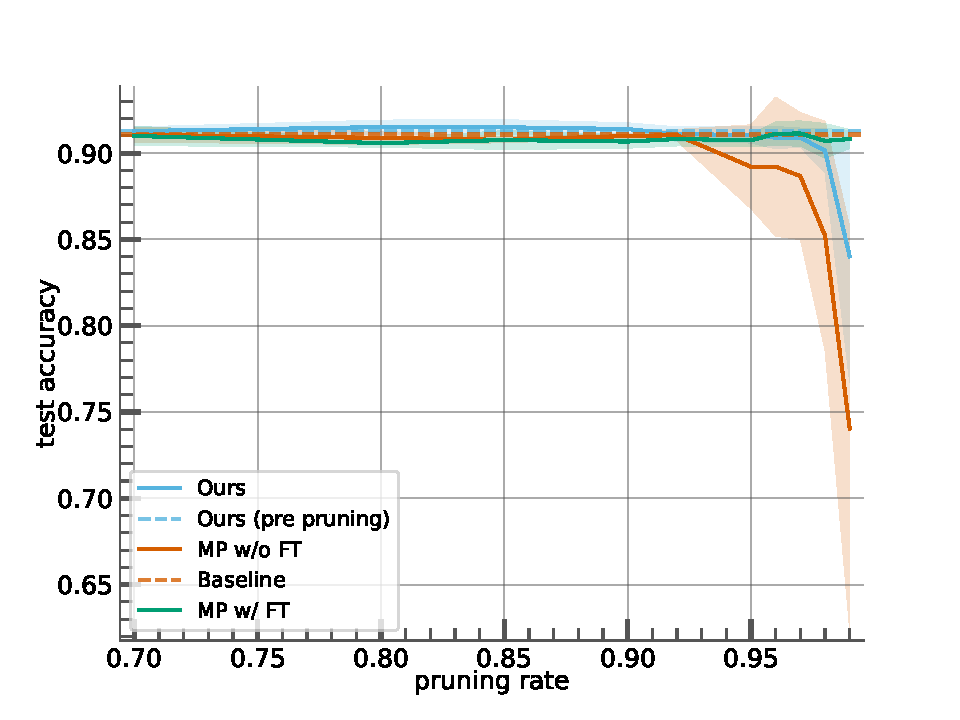
\includegraphics[width=0.49\linewidth]{chapter_1/assets/reparam_vs_mpft_PrunableVGG16_cifar10.pdf}
      \label{fig:chap1:reparam_vs_mpft_vgg16_cifar10}} 
  \subfloat[VGG16 - CIFAR100]{
      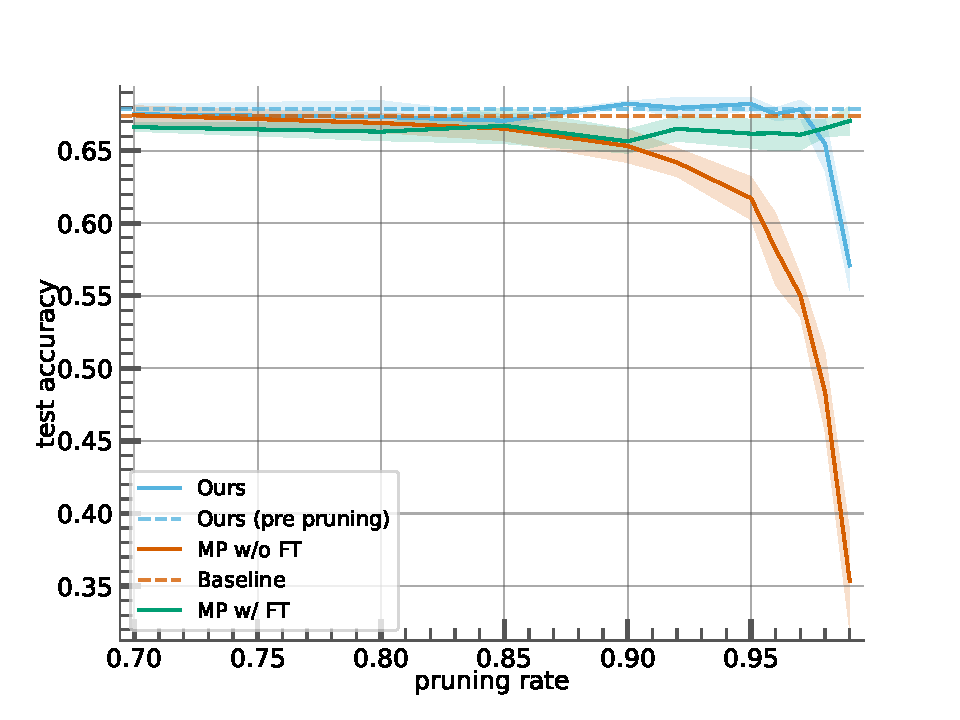
\includegraphics[width=0.49\linewidth]{chapter_1/assets/reparam_vs_mpft_PrunableVGG16_cifar100.pdf}
      \label{fig:chap1:reparam_vs_mpft_vgg16_cifar100}} 
  \\
  \subfloat[VGG16 - CIFAR10 (Number of Epochs)\label{fig:chap1:reparam_vs_mpft_vgg16_cifar10_epochs}]{
    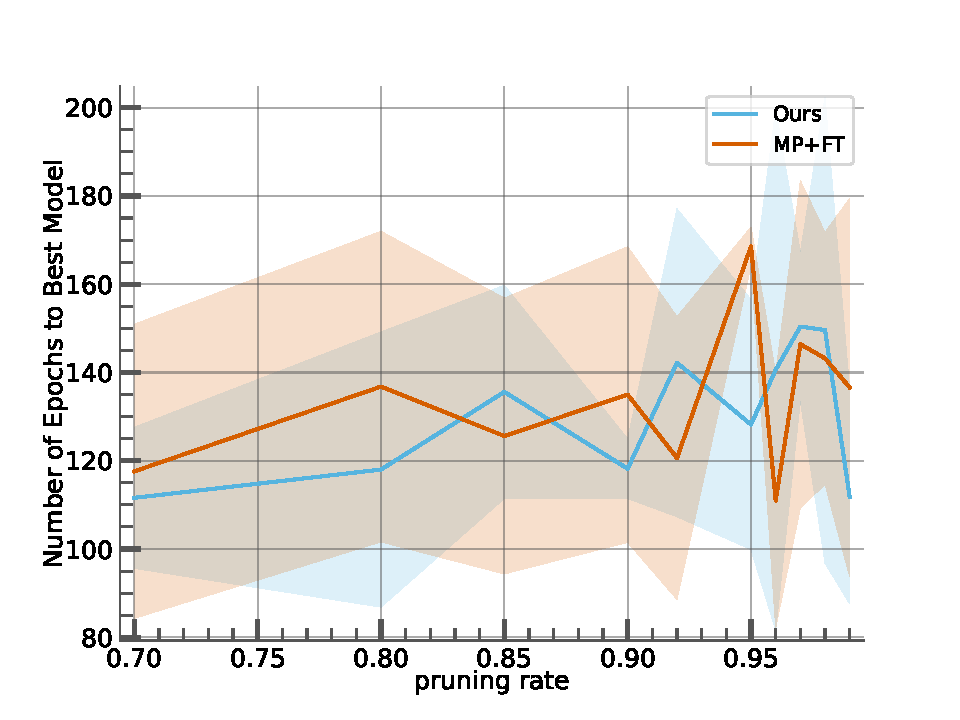
\includegraphics[width=0.49\linewidth]{chapter_1/assets/reparam_vs_mpft_training_time_PrunableVGG16_cifar10.pdf}}
  \subfloat[VGG16 - CIFAR100 (Number of Epochs)\label{fig:chap1:reparam_vs_mpft_vgg16_cifar100_epochs}]{
      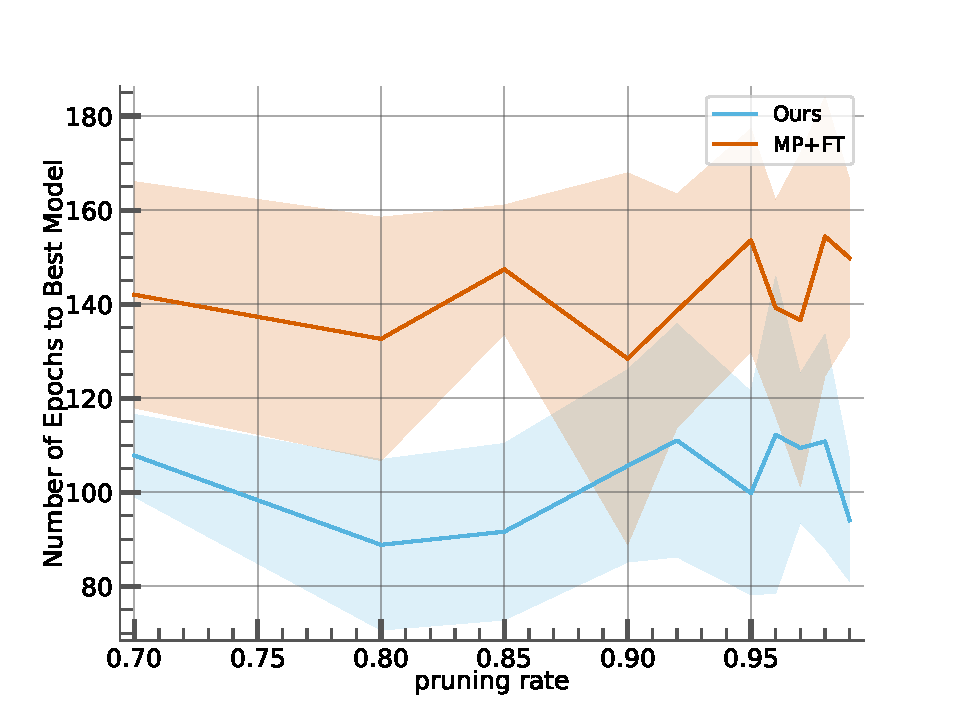
\includegraphics[width=0.49\linewidth]{chapter_1/assets/reparam_vs_mpft_training_time_PrunableVGG16_cifar100.pdf}}

    
  \caption{ Performances comparison of our method \em{(Ours)} against
  magnitude pruning with fine-tuning \em{(MP+FT)} with a VGG16 network on
  CIFAR10 and CIFAR100 datasets, for different pruning rates.
  \Cref{fig:chap1:reparam_vs_mpft_vgg16_cifar10} and
  \cref{fig:chap1:reparam_vs_mpft_vgg16_cifar100} show the testing accuracy of
  the model and \cref{fig:chap1:reparam_vs_mpft_vgg16_cifar10_epochs} and
  \cref{fig:chap1:reparam_vs_mpft_vgg16_cifar100_epochs} the
  number of epochs needed to obtain the best model.}
  \label{fig:chap1:reparam_vs_mpft_vgg16}
\end{figure}

\begin{figure}
  \centering
  \subfloat[ResNet20 - CIFAR10\label{fig:chap1:reparam_vs_mpft_resnet20_cifar10}]{
      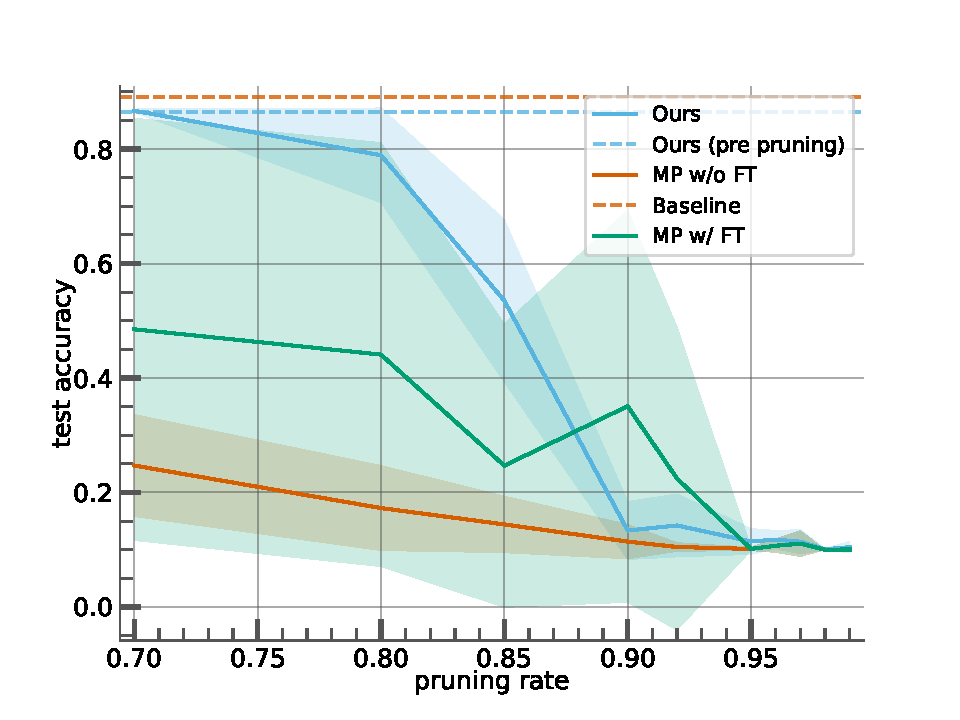
\includegraphics[width=0.49\linewidth]{chapter_1/assets/reparam_vs_mpft_PrunableResNet20_cifar10.pdf}}
  \subfloat[ResNet20 - CIFAR100\label{fig:chap1:reparam_vs_mpft_resnet20_cifar100}]{
      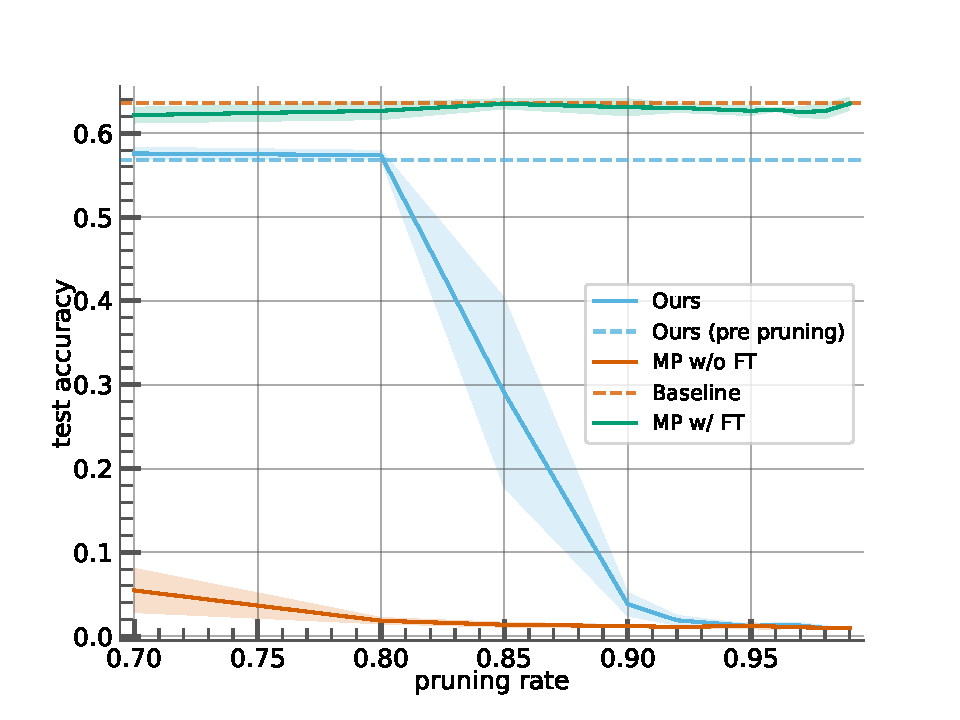
\includegraphics[width=0.49\linewidth]{chapter_1/assets/reparam_vs_mpft_PrunableResNet20_cifar100.pdf}} 
  \\
  \subfloat[ResNet20 - CIFAR10 (Number of Epochs)\label{fig:chap1:reparam_vs_mpft_resnet20_cifar10_epochs}  ]{
      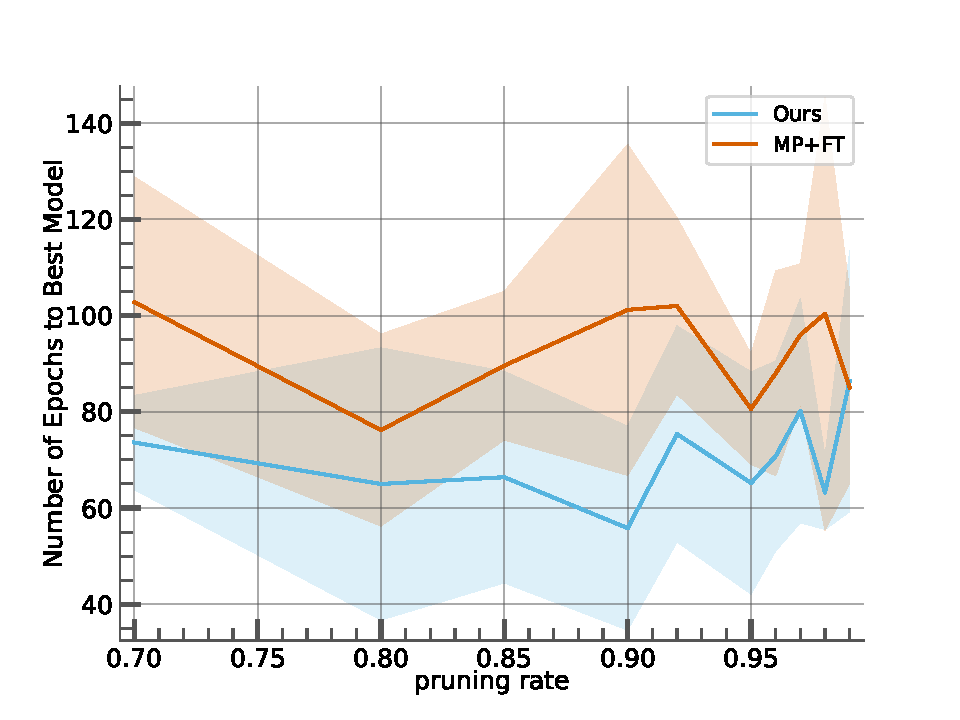
\includegraphics[width=0.49\linewidth]{chapter_1/assets/reparam_vs_mpft_training_time_PrunableResNet20_cifar10.pdf}}
  \subfloat[ResNet20 - CIFAR100 (Number of Epochs)\label{fig:chap1:reparam_vs_mpft_resnet20_cifar100_epochs}]{
      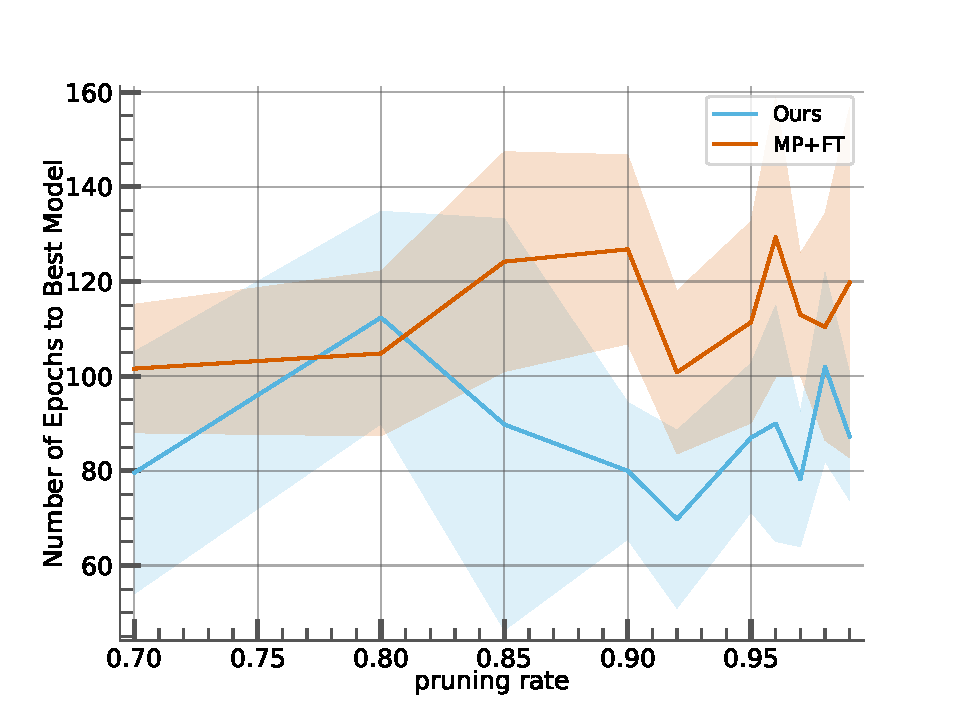
\includegraphics[width=0.49\linewidth]{chapter_1/assets/reparam_vs_mpft_training_time_PrunableResNet20_cifar100.pdf}}
  \caption{ Performances comparison of our method \em{(Ours)} against
  magnitude pruning with fine-tuning \em{(MP+FT)} with a ResNet20 network on
  CIFAR10 and CIFAR100 datasets, for different pruning rates.
  \Cref{fig:chap1:reparam_vs_mpft_resnet20_cifar10} and
  \cref{fig:chap1:reparam_vs_mpft_resnet20_cifar100} show the
  testing accuracy of the model and
  \cref{fig:chap1:reparam_vs_mpft_resnet20_cifar10_epochs} and
  \cref{fig:chap1:reparam_vs_mpft_resnet20_cifar100_epochs}
  the number of epochs needed to obtain the best model.}
  \label{fig:chap1:reparam_vs_mpft_resnet20}
\end{figure}


\begin{figure}
  \centering
  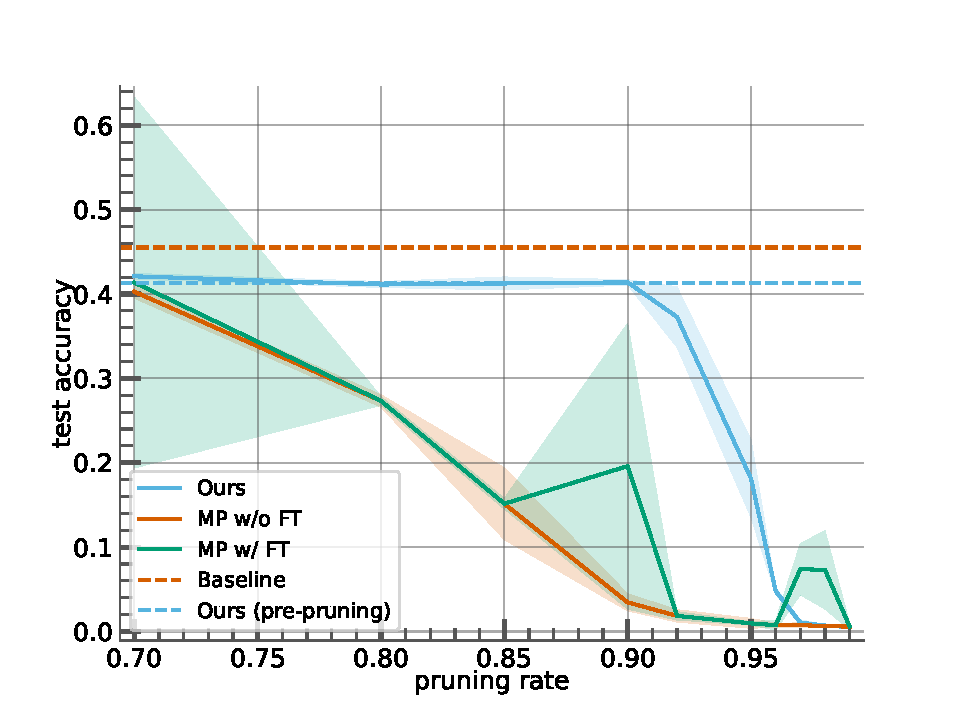
\includegraphics[width=0.49\textwidth]{chapter_1/assets/reparam_vs_mpft_PrunableResNet18_tinyimagenet.pdf}
  \caption{Performances comparison of our method \em{(Ours)} against
  magnitude pruning with fine-tuning \em{(MP+FT)} with a ResNet18 network on
  TinyImageNet dataset, for different pruning rates.}
  \label{fig:chap1:reparam_vs_mpft_resnet18}
\end{figure}

% endregion: perfs_figures

\subsection{Optimal value of \texorpdfstring{$\lambda$}{Lambda}}
\label{sec:chap1:impact_of_lambda}
Our method relies on a budget loss which relative importance compared to the
main task loss is controlled by a parameter $\lambda$ (cf.
\cref{eqn:chap1:globalloss}). The choice of this parameter is crucial to ensure
a good tradeoff between \emph{(i)} the respect of the budget, in order to
mitigate the performance drop following the effective pruning step; and
\emph{(ii)} the optimisation of the main task loss, which influences the final
performance. The achieved budget as a function of the parameter $\lambda$ is
detailed for different pruning rates in
\cref{fig:chap1:lambda_impact_pruning_90,fig:chap1:lambda_impact_pruning_95,fig:chap1:lambda_impact_pruning_99}.
In these figures, the achieved budget is computed as the sum of the weights reparametrisation\\

For low pruning rates (\cref{fig:chap1:lambda_impact_pruning_90}), a low value
of $\lambda$ does not enforce the respect of the budget and in this case, the
final network has a smaller achieved budget than the targeted one. Similarly,
for higher pruning rates (\cref{fig:chap1:lambda_impact_pruning_99}), a low
value of $\lambda$ results in a budget in excess compared to the targeted one.
In both cases, the performances of networks trained with a low value of
$\lambda$ are subpar compared to higher values, as reported in
\cref{tab:chap1:lambda_impact}. On the opposite of the spectrum, high values of
$\lambda$ lay too much emphasis on the budget loss, and the network performances
are negatively impacted, even though the budget is respected. Following the
abovementioned considerations, we set the value of $\lambda$ to 5 for all the
experiments. This value strikes the best balance between the two objectives:
budget loss and main task loss.

% region: lambda_impact_figures

\begin{figure}
  \centering
  \subfloat[Pruning 90\% of the weights\label{fig:chap1:lambda_impact_pruning_90}]{
    
\includegraphics[width=0.49\linewidth]{chapter_1/assets/lambda_impact_pr_90_C4_CIFAR10.pdf}}
  \subfloat[Pruning 95\% of the weights\label{fig:chap1:lambda_impact_pruning_95}]{
    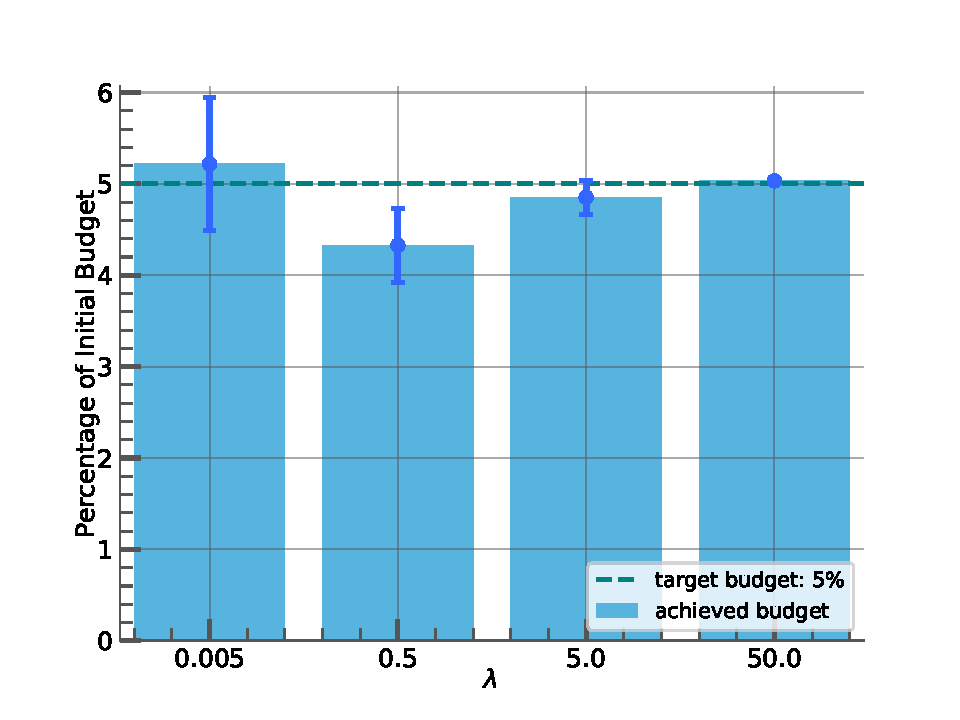
\includegraphics[width=0.49\linewidth]{chapter_1/assets/lambda_impact_pr_95_C4_CIFAR10.pdf}}
  \\
  \subfloat[Pruning 99\% of the weights\label{fig:chap1:lambda_impact_pruning_99}]{
    
\includegraphics[width=0.49\linewidth]{chapter_1/assets/lambda_impact_pr_99_C4_CIFAR10.pdf}}
    \caption{ Impact of the parameter $\lambda$ on the achieved final
    budget for a Conv4 network on CIFAR10 dataset, for various pruning rates. A
    too-small value of $\lambda$ does not make the actual budget match the desired
    budget. The actual budget is either too small
    (\cref{fig:chap1:lambda_impact_pruning_90}) or too high
    (\cref{fig:chap1:lambda_impact_pruning_99}) compared to the target, depending
    on the applied pruning rate.}
  \label{fig:chap1:lambda_impact}
  \end{figure}  


\begin{table}[tbp]
  \centering
  \begin{center}
    \begin{tabular}{llcc}
      \toprule
      \textbf{Pruning Rate} & \textbf{$\lambda$} & \textbf{Achieved Budget} & \textbf{Test Accuracy (post pruning)} \\
      \midrule
      \multirow{4}{*}{0.9} & 0.005 & 5.25 $\pm$ 0.69 & 85.83 $\pm$ 0.83 \\
      & 0.5 & 8.06 $\pm$ 0.19 & 86.34 $\pm$ 0.64 \\
      & 5 & 9.93 $\pm$ 0.03 & 85.82 $\pm$ 0.74 \\
      & 50 & \textbf{10.00 $\pm$ 0.01} & \textbf{86.52 $\pm$ 0.46} \\
      \midrule
      \multirow{4}{*}{0.95} & 0.005 & 5.22 $\pm$ 0.73 & \textbf{86.27 $\pm$ 0.32} \\
      & 0.5 & 4.33 $\pm$ 0.41 & 85.66 $\pm$ 0.74 \\
      & 5 & 4.85 $\pm$ 0.19 & 86.11 $\pm$ 0.48 \\
      & 50 & \textbf{5.03 $\pm$ 0.02} & 85.37 $\pm$ 0.37 \\
      \midrule
      \multirow{4}{*}{0.99} & 0.005 & 4.60 $\pm$ 0.29 & 40.52 $\pm$ 5.27 \\
      & 0.5 & 3.69 $\pm$ 0.38 & 42.45 $\pm$ 9.02 \\
      & 5 & 1.89 $\pm$ 0.45 & \textbf{76.85 $\pm$ 6.34} \\
      & 50 & \textbf{2.09 $\pm$ 0.15} & 10.00 $\pm$ 0.00 \\
      \bottomrule
    \end{tabular}
  \end{center}
  \caption{
    Impact of the parameter $\lambda$ on the achieved budget and the post-pruning test accuracy of the model for a Conv4 network on the CIFAR10 dataset
    for various pruning rates. Although a high value of $\lambda$ ensures 
    the target budget is reached, it also leads to a lower test accuracy when
    the pruning rate increases.}
    \label{tab:chap1:lambda_impact}
\end{table}

% endregion: lambda_impact_figures

\subsection{Impact of the budget loss}
\label{sec:chap1:impact_of_budget_loss}
To establish the importance and the efficacy of the budget loss in our method,
we present in this section the results of a comparative experimental analysis
with alternative variants.  Specifically, we investigated the impact of the
budget loss by comparing it with two other variants: \emph{(i)} a variant where the
budget loss was removed, and \emph{(ii)} a variant where the budget loss is replaced
with an $L_1$ regularisation loss on the network weights. To remove the budget
loss, the value of $\lambda$ is set to zero 0 in \cref{eqn:chap1:globalloss}. In the
second variant, we varied the mixing coefficient $\lambda$ between 0.1 and 100.
Considering the same issue of loss conditioning as in
\cref{sec:chap1:budget_loss}, the $L_1$ loss is divided by the total number of
parameters before being added to the global loss. This specific global loss is
expressed as:

\begin{equation}
  \label{eqn:chap1:globalloss_l1}
  \mathcal{L} = \mathcal{L}_{task} + \lambda \cdot \frac{1}{N} \sum_{i=1}^{N} \left| w_i \right|
\end{equation}

Where $|~.~|$ represents the absolute value, and $N$ is the total number of
parameters in the network (as reported in \cref{tab:chap1:networks_size}).\\

In both variants, the reparametrisation is kept in order to isolate the impact
of the budget loss. We evaluated the performance of our approach and the two
variants on the CIFAR10 and CIFAR100 datasets using Conv4, VGG16, and ResNet20
networks. The results are presented in
\cref{fig:chap1:no_budget_conv4,fig:chap1:no_budget_resnet20,fig:chap1:no_budget_vgg16}.
In the figures mentioned above, the variant without the budget loss is denoted
\emph{w/o budget}, and the variant with a $L_1$ regularisation loss is referred
as \emph{$L_1$ reg.}. The results denoted \emph{w/ budget} represents our method
in the same setup as in \cref{sec:chap1:performances}.\\

Removing the budget loss (variant \emph{(i)}) negatively impacts the network
performances. The test accuracy is systematically lower than the one obtained
with the budget loss. This is particularly visible in
\cref{fig:chap1:no_budget_conv4_cifar100,fig:chap1:no_budget_vgg16_cifar100}.
Removing the budget loss does not allow to introduce sparsity, much less to
respect a target budget. Therefore, effective pruning impacts all the more
negatively the network performance since it was not trained with a prior on
either sparsity or budget. \\

Replacing the budget loss with a $L_1$ regularisation loss (variant \emph{(ii)})
also impacts negatively the performance, with the exception of the ResNet20
network (\cref{fig:chap1:no_budget_resnet20}). Although performances are
generally worse than our method (\emph{w/ budget}), results indicate that the
mixing coefficient $\lambda$ has a major importance. Indeed, the $L_1$
regulatisation does not target a precise budget, however, it still introduces
sparsity in the network. Thus, for certain pruning rates, the variant
\emph{(ii)} can exhibit better results than our method (especially visible on
\cref{fig:chap1:no_budget_resnet20_cifar10,fig:chap1:no_budget_resnet20_cifar100}).
Nevertheless, the choice of $\lambda$ is critial and not trivial. Because of the
absence of a budget loss, the level of sparsity is to be controlled only by the
parameter $\lambda$, which makes it difficult to find a single value suited for
a large range of pruning rates, networks and datasets.\\

In contrast, our method is able to achieve good performance accross multiple and
diverse conditions, without the need to fine-tune the value of $\lambda$.
Experiments presented in this section reveal that the budget loss is a critical
component of the method to train networks and prune them while introducing a
minimal impact on the performance if no fine-tuning is applied. While the $L_1$
regularisation loss may achieve superior performance in certain cases, our
method is more straightforward and robust in its applicability across various
scenarios.\\

% region: no budget
\begin{figure}
  \centering
  \subfloat[Conv4 CIFAR10\label{fig:chap1:no_budget_conv4_cifar10}]{
    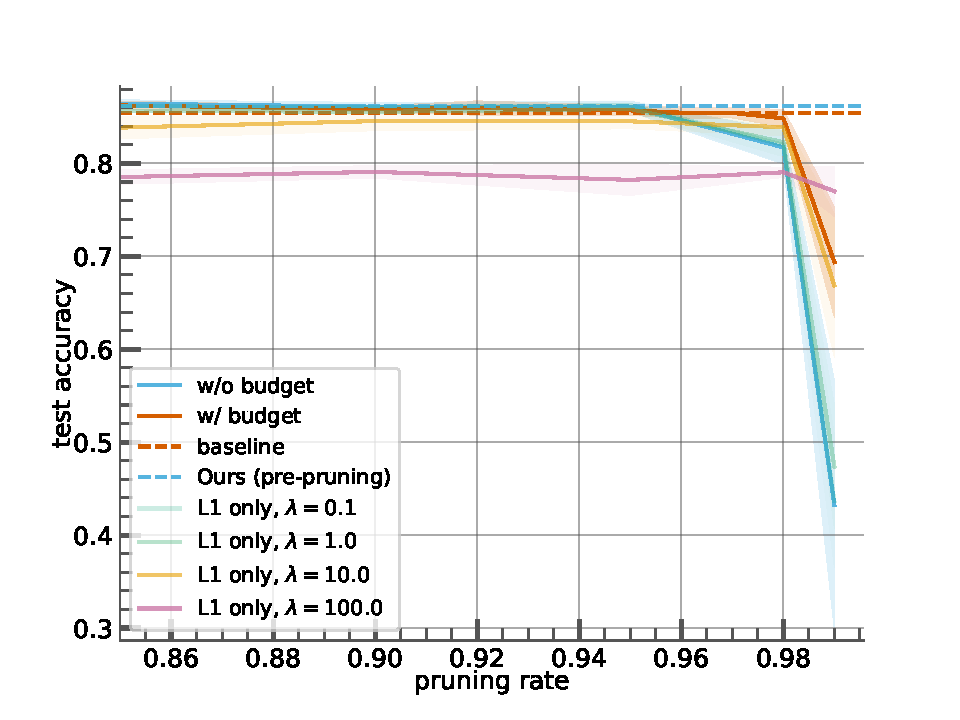
\includegraphics[width=0.49\textwidth]{chapter_1/assets/ours_vs_no_lambda_vs_l1_only_cifar10_Conv4.pdf}}
    \subfloat[Conv4 CIFAR100\label{fig:chap1:no_budget_conv4_cifar100}]{
    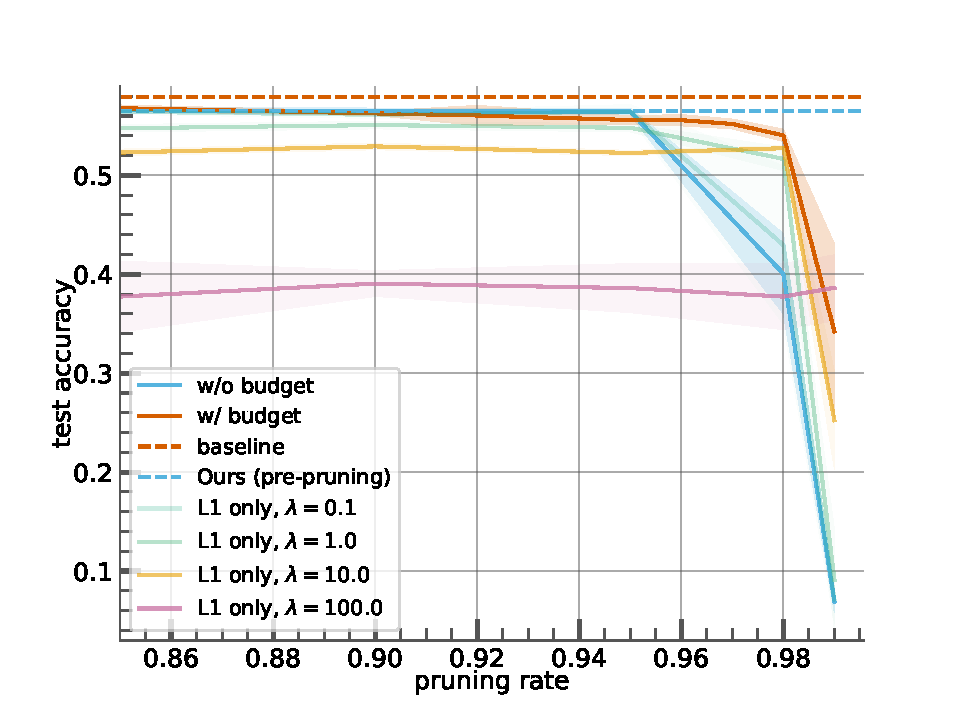
\includegraphics[width=0.49\textwidth]{chapter_1/assets/ours_vs_no_lambda_vs_l1_only_cifar100_Conv4.pdf}}
    \caption{ Comparison of our method and its variant without the
    budget loss. The experimental results are denoted \emph{$L_1$ reg.}, wherein
    the budget loss is replaced by a $L_1$ regularisation loss on the network
    weights. The mixing coefficient $\lambda$ is varied from 0.1 to 100,
    depending on the experiment. \emph{w/o budget} denotes the absence of the
    budget loss (this is equivalent to $\lambda = 0$). On the other hand,
    \emph{w/ budget} corresponds to our method, with the same setup as described
    in \cref{sec:chap1:performances}. Results are presented for a Conv4 network,
    trained on CIFAR10 (\cref{fig:chap1:no_budget_conv4_cifar10}) and CIFAR100
    (\cref{fig:chap1:no_budget_conv4_cifar100})} 
      \label{fig:chap1:no_budget_conv4}
\end{figure}
  
  

\begin{figure}
  \centering
  \subfloat[ResNet20 CIFAR10\label{fig:chap1:no_budget_resnet20_cifar10}]{
    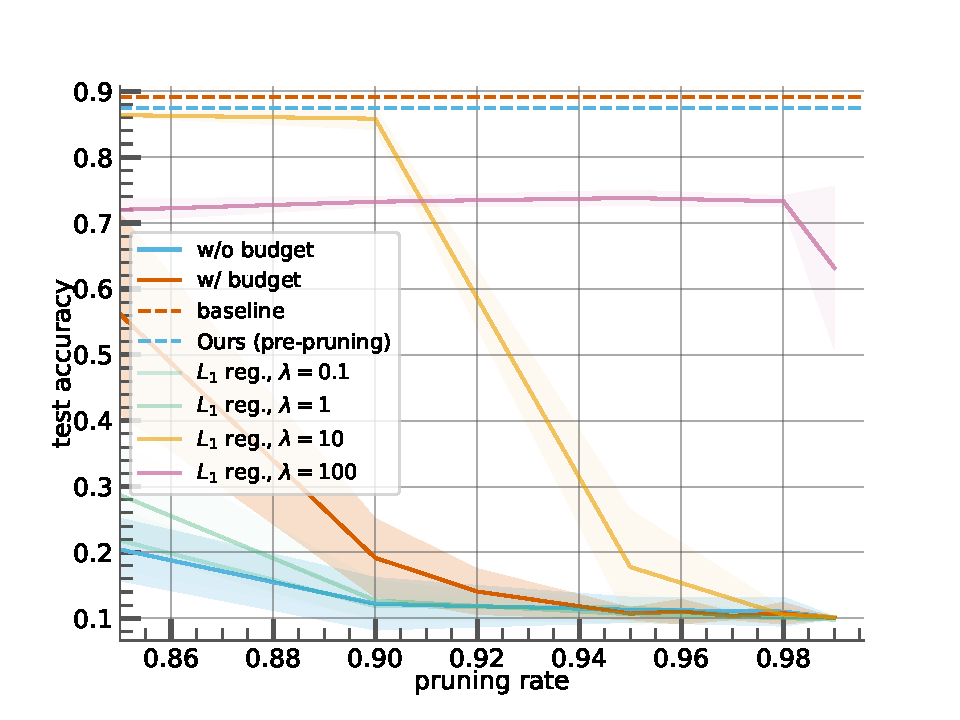
\includegraphics[width=0.49\textwidth]{chapter_1/assets/ours_vs_no_lambda_vs_l1_only_cifar10_PrunableResNet20.pdf}}
    \subfloat[ResNet20 CIFAR100\label{fig:chap1:no_budget_resnet20_cifar100}]{
    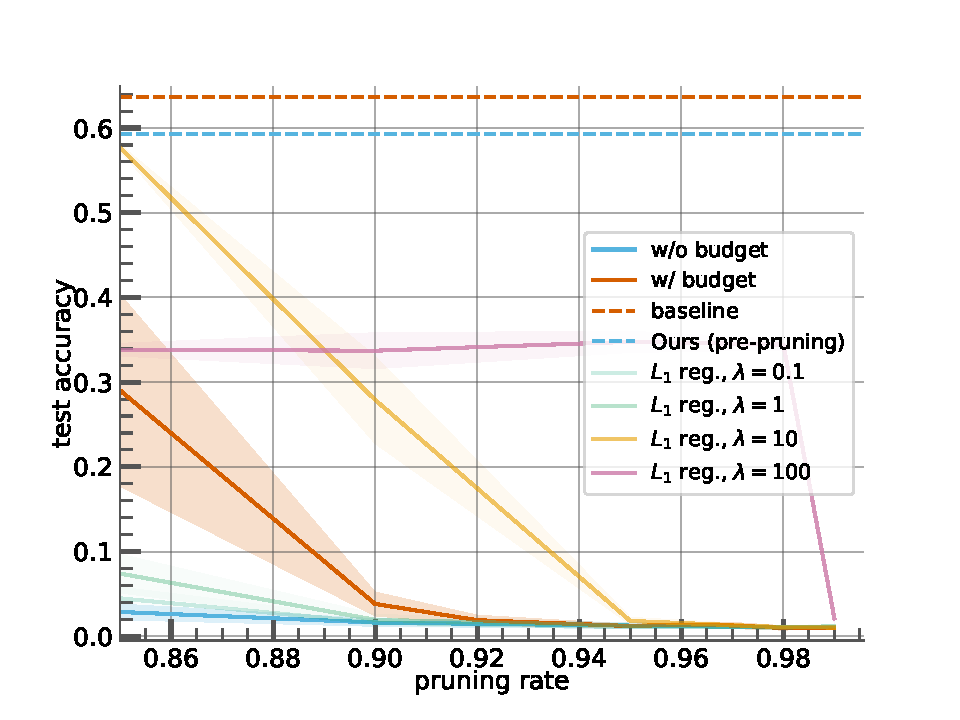
\includegraphics[width=0.49\textwidth]{chapter_1/assets/ours_vs_no_lambda_vs_l1_only_cifar100_PrunableResNet20.pdf}}
    \caption{ Comparison of our method and its variant without the
    budget loss. The experimental results are denoted \emph{$L_1$ reg.}, wherein
    the budget loss is replaced by a $L_1$ regularisation loss on the network
    weights. The mixing coefficient $\lambda$ is varied from 0.1 to 100,
    depending on the experiment. \emph{w/o budget} denotes the absence of the
    budget loss (this is equivalent to $\lambda = 0$). On the other hand,
    \emph{w/ budget} corresponds to our method, with the same setup as described
    in \cref{sec:chap1:performances}. Results are presented for a ResNet20
    network, trained on CIFAR10 (\cref{fig:chap1:no_budget_resnet20_cifar10})
    and CIFAR100 (\cref{fig:chap1:no_budget_resnet20_cifar100})}       
    \label{fig:chap1:no_budget_resnet20}
\end{figure}
  
    

\begin{figure}
  \centering
  \subfloat[VGG16 CIFAR10\label{fig:chap1:no_budget_vgg16_cifar10}]{
    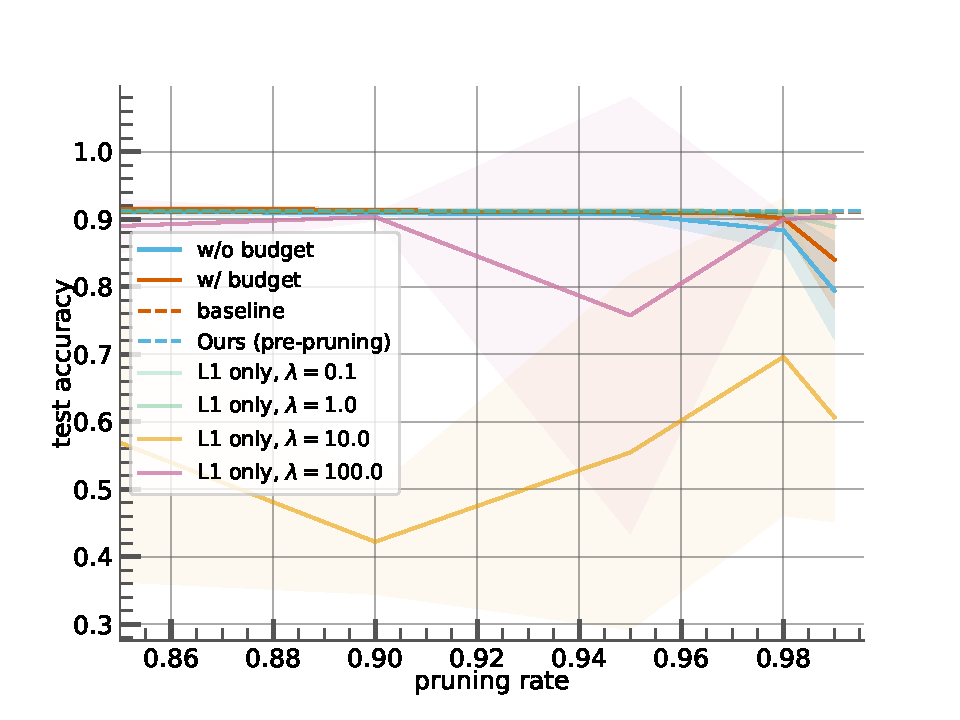
\includegraphics[width=0.49\textwidth]{chapter_1/assets/ours_vs_no_lambda_vs_l1_only_cifar10_PrunableVGG16.pdf}}
    \subfloat[VGG16 CIFAR100\label{fig:chap1:no_budget_vgg16_cifar100}]{
    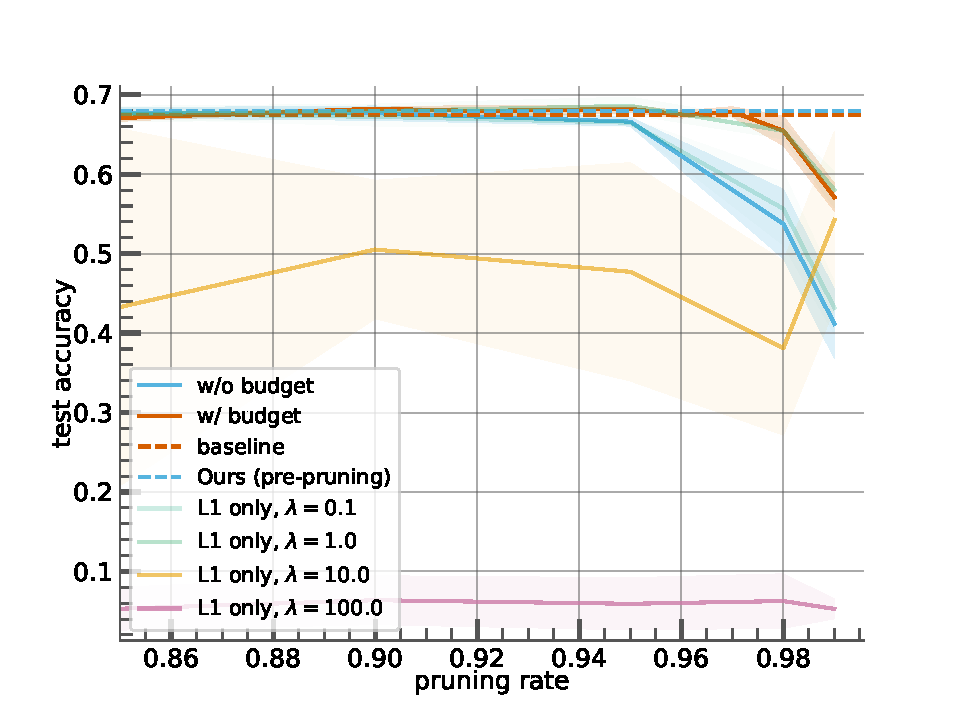
\includegraphics[width=0.49\textwidth]{chapter_1/assets/ours_vs_no_lambda_vs_l1_only_cifar100_PrunableVGG16.pdf}}
    \caption{ Comparison of our method and its variant without the
    budget loss. The experimental results are denoted \emph{$L_1$ reg.}, wherein
    the budget loss is replaced by a $L_1$ regularisation loss on the network
    weights. The mixing coefficient $\lambda$ is varied from 0.1 to 100,
    depending on the experiment. \emph{w/o budget} denotes the abscence of the
    budget loss (this is equivalent to $\lambda = 0$). On the other hand,
    \emph{w/ budget} corresponds to our method, with the same setup as described
    in \cref{sec:chap1:performances}. Results are presented for a VGG16 network,
    trained on CIFAR10 (\cref{fig:chap1:no_budget_vgg16_cifar10}) and CIFAR100
    (\cref{fig:chap1:no_budget_vgg16_cifar100})}       
    \label{fig:chap1:no_budget_vgg16}
\end{figure}

% endregion: no budget

\subsection{Impact of the reparametrisation}
\label{sec:chap1:impact_of_reparametrisation}

The proposed method comprises two primary components: budget loss and weight
reparametrization. The previous section establishes the significance of the
budget loss in achieving optimal performance. In this section, we present the
cruciality of incorporating weight reparametrization. To establish the necessity
of weight reparametrisation, we compare our approach with a variant where the
budget loss is applied but the weight reparametrisation is not. This variant is
denoted \emph{budget only} in the following. The objective of this variant and
the comparison is to isolate the impact of weight reparametrization.\\


We evaluate the performance of our method and the \emph{budget only} variant on
Conv4, ResNet20, and VGG16 networks using CIFAR10 and CIFAR100 datasets (see
\Cref{fig:chap1:budget_only_conv4,fig:chap1:budget_only_resnet20,fig:chap1:budget_only_resnet20}).
Both the proposed approach and \emph{budget only} variant are trained with the
same hyperparameters. Among other things, the mixing coefficient $\lambda$ is
set to 5. We perform experiments by varying $\lambda$ from 0.5 to 50, but the
results are almost identical and the lines are indistinguishable. Therefore, we
show the results only for $\lambda = 5$ to maintain figure clarity.\\

\Cref{fig:chap1:budget_only_conv4,fig:chap1:budget_only_resnet20,fig:chap1:budget_only_resnet20}
present the results of the performance comparison. Our method is denoted as
\emph{budget + reparam} and is evaluated after pruning, whereas the \emph{budget
nly} variant's results are presented both before and after pruning. On Conv4 and
VGG16 (\cref{fig:chap1:budget_only_conv4,fig:chap1:budget_only_vgg16},
respectively), our method performs on par with the \emph{budget only} variant
before pruning while being already pruned, up to very high pruning rates (more
than 98\%). On the contrary, and even for ResNet20, the \emph{budget only}
post-pruning variant performs poorly. The \emph{budget only} variant performance
is massively impaired by the \emph{effective pruning} step, even though the
budget is thoroughly respected (\cref{tab:chap1:impact_of_reparametrisation}).
In comparison, our method performs much better when both methods are pruned. The
budget loss alone enforces a stricter adherence to the target budget
(\cref{tab:chap1:impact_of_reparametrisation}), however, the lack of
reparametrisation fails to prepare the network for the \emph{effective pruning}
step. Indeed, weights are not soft-pruned and the network is not prepared for sparsity.\\

\begin{table}
\centering
\begin{tabular}{lllc}
  \toprule
  \textbf{Dataset} & \textbf{Network} & \textbf{Pruning Rate} & \textbf{Achieved Budget} \\
  \midrule
  \multirow{9}{*}{CIFAR10} & \multirow{3}{*}{Conv4} & 0.9 & 9.99 $\pm$ 0.00 \\
     &  & 0.95 & 4.97 $\pm$ 0.01 \\
     &  & 0.99 & 0.98 $\pm$ 0.00 \\
     \cline{2-4}
   & \multirow{3}{*}{ResNet20} & 0.9 & 9.83 $\pm$ 0.02 \\
     &  & 0.95 & 4.88 $\pm$ 0.01 \\
     &  & 0.99 & 0.98 $\pm$ 0.00 \\
     \cline{2-4}

   & \multirow{3}{*}{VGG16} & 0.9 & 10.00 $\pm$ 0.00 \\
     &  & 0.95 & 5.00 $\pm$ 0.00 \\
    &  & 0.99 & 1.00 $\pm$ 0.00 \\
    \midrule
  \multirow{9}{*}{CIFAR100} & \multirow{3}{*}{Conv4} & 0.9 & 9.94 $\pm$ 0.02 \\
     &  & 0.95 & 4.91 $\pm$ 0.02 \\
    &  & 0.99 & 0.98 $\pm$ 0.00 \\
    \cline{2-4}

   & \multirow{3}{*}{ResNet20} & 0.9 & 9.84 $\pm$ 0.02 \\
     &  & 0.95 & 4.91 $\pm$ 0.01 \\
     &  & 0.99 & 1.00 $\pm$ 0.00 \\
     \cline{2-4}

   & \multirow{3}{*}{VGG16} & 0.9 & 10.00 $\pm$ 0.00 \\
     &  & 0.95 & 5.00 $\pm$ 0.00 \\
    &  & 0.99 & 1.00 $\pm$ 0.00 \\
  \bottomrule
  \end{tabular}
  \caption{Achieved budget for the \emph{budget only} variant. Results are
  presented for $\lambda=5$. Across all experiments, the achieved budget matches
  closely the targeted budget (computed as $1-$pruning
  rate).}
  \label{tab:chap1:impact_of_reparametrisation}
\end{table}

The results presented in this comparison and the one of
\cref{sec:chap1:budget_loss} indicate that both components of our method are of
crucial importance. In particular, the reparametrization allows for a
considerably better generalization of the network after pruning, thus enabling a
much higher level of performance.
\Cref{sec:chap1:impact_of_budget_loss,sec:chap1:impact_of_reparametrisation}
demonstrate experimentally that no component of our method can be removed
without significant impairment of the performance, and therefore, they
function in synergy.

% region: budget only

\begin{figure}
\centering
  \subfloat[Conv4 CIFAR10\label{fig:chap1:budget_only_conv4_cifar10}]{
  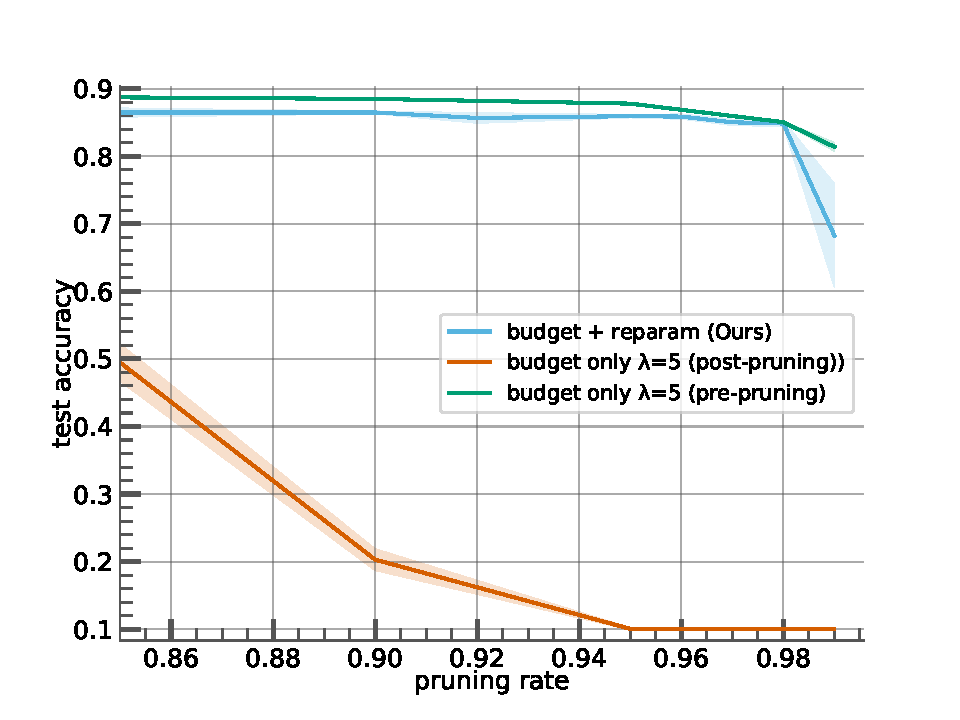
\includegraphics[width=0.49\textwidth]{chapter_1/assets/budget_only_cifar10_Conv4.pdf}}
  \subfloat[Conv4 CIFAR100\label{fig:chap1:budget_only_conv4_cifar100}]{
  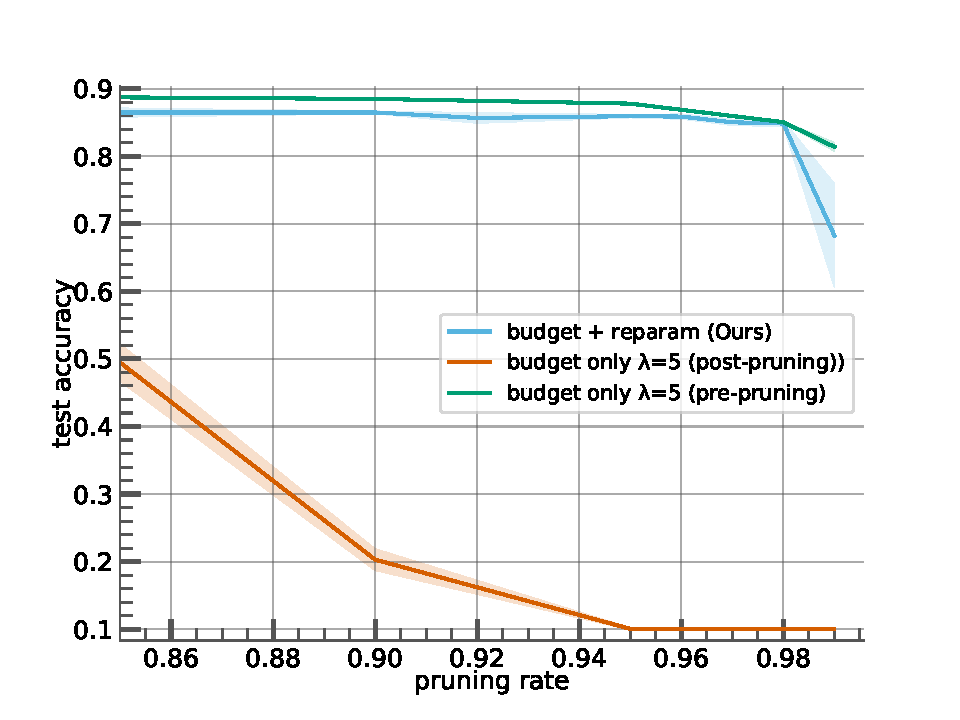
\includegraphics[width=0.49\textwidth]{chapter_1/assets/budget_only_cifar10_Conv4.pdf}}
  \caption{Comparison of our method and its variant without the
  reparametrization on Conv4, evaluated on CIFAR10 and CIFAR100. Our method
  (\emph{budget + reparam}) has similar performance to the \emph{budget only}
  variant before pruning, whereas our method, is already pruned. Once pruned,
  the \emph{budget only} variant is significantly impaired.}
  \label{fig:chap1:budget_only_conv4}
\end{figure}

\begin{figure}
  \centering
  \subfloat[ResNet20 CIFAR10\label{fig:chap1:budget_only_resnet20_cifar10}]{
  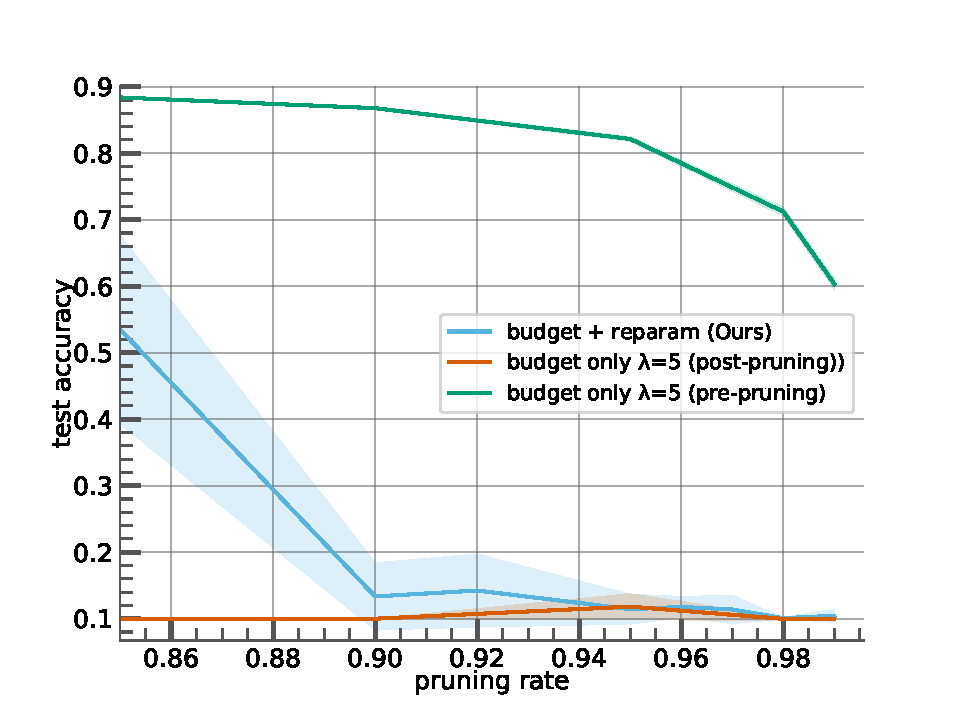
\includegraphics[width=0.49\textwidth]{chapter_1/assets/budget_only_cifar10_PrunableResNet20.pdf}}
  \subfloat[ResNet20 CIFAR100\label{fig:chap1:budget_only_resnet20_cifar100}]{
  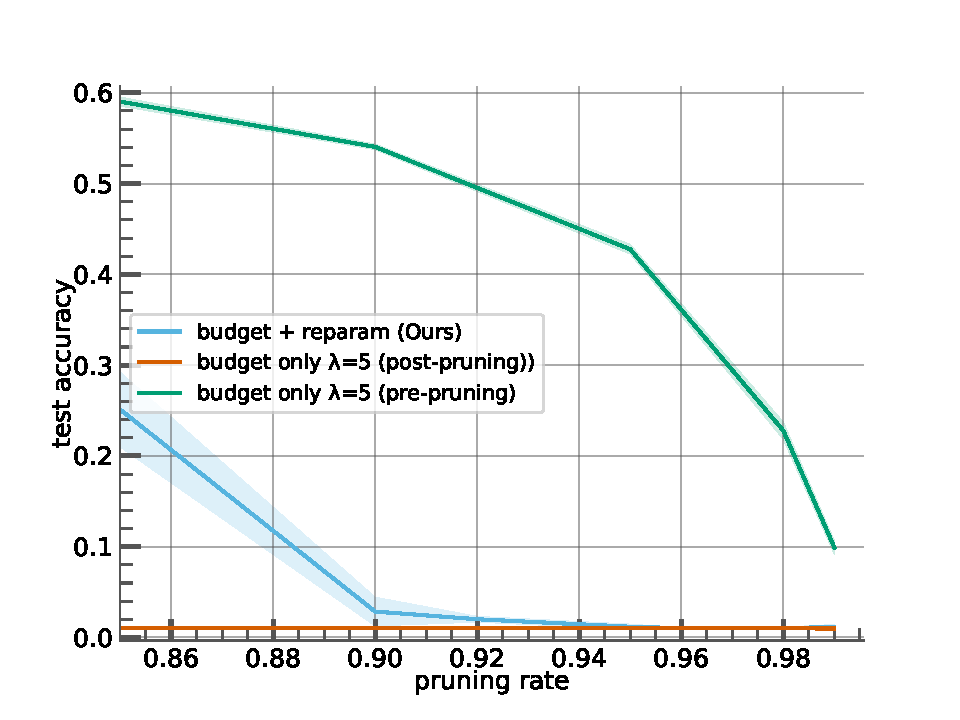
\includegraphics[width=0.49\textwidth]{chapter_1/assets/budget_only_cifar100_PrunableResNet20.pdf}}
  \caption{Comparison of our method and its variant without the
  reparametrization on ResNet20, evaluated on CIFAR10 and CIFAR100. Due to the
  small size of the network (see \cref{tab:chap1:networks_size}), the pruned
  version of our method (\emph{budget + reparam}) and the \emph{budget only}
  variant cannot keep up with the unpruned version. Nevertheless, if considering
  the pruned versions, our method scores better, thanks to the addition of the
  reparametrization.}
  \label{fig:chap1:budget_only_resnet20}
\end{figure}

\begin{figure}
  \centering
  \subfloat[VGG16 CIFAR10\label{fig:chap1:budget_only_vgg6_cifar10}]{
  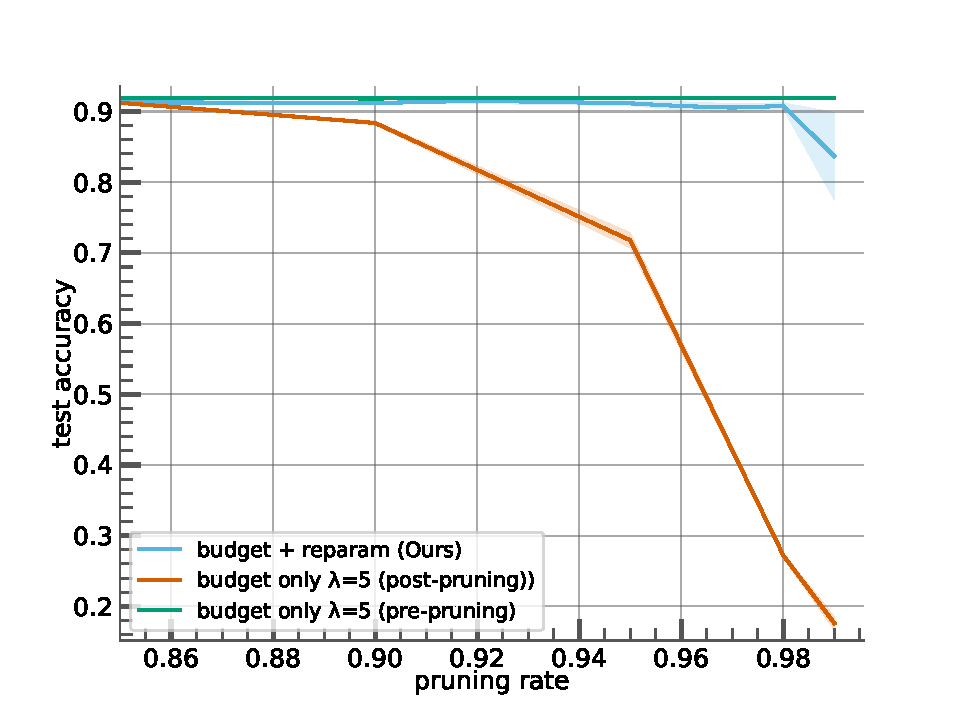
\includegraphics[width=0.49\textwidth]{chapter_1/assets/budget_only_cifar10_PrunableVGG16.pdf}}
  \subfloat[VGG16 CIFAR100\label{fig:chap1:budget_only_vgg6_cifar100}]{
  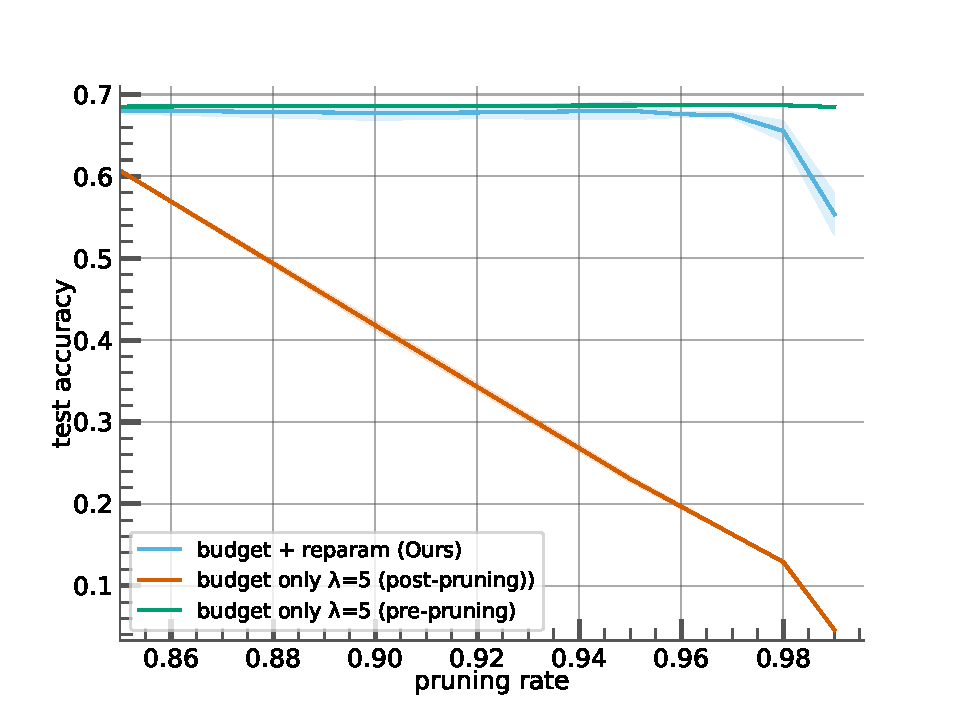
\includegraphics[width=0.49\textwidth]{chapter_1/assets/budget_only_cifar100_PrunableVGG16.pdf}}
  \caption{Comparison of our method and its variant without the
  reparametrizationn VGG16, evaluated on CIFAR10 and CIFAR100. Our method
  (\emph{budget + reparam}) has similar performance to the \emph{budget only}
  variant before pruning, whereas our method, is already pruned. Once pruned,
  the \emph{budget only} variant is significantly impaired.}
  \label{fig:chap1:budget_only_vgg16}
\end{figure}

% endregion: budget only

\subsection{Fine-tuning context}
\label{sec:chap1:impact_of_fine_tuning}

Although the method presented in this chapter was designed from the ground up to
circumvent the need for fine-tuning, it can be used to fine-tune a network
trained conventionally. In this section, we compare the performances of a
network trained in a standard way, pruned and then fine-tuned with two methods:
Our method and standard fine-tuning \cite{DBLP:conf/nips/HanPTD15}. This setup
is evaluated on Conv4, ResNet20 and VGG16 for both CIFAR10 and CIFAR100. The
results are shown in 
\cref{fig:chap1:finetuning_impact_conv4,fig:chap1:finetuning_impact_resnet20,fig:chap1:finetuning_impact_vgg6}.
First, a network is trained for 150 epochs on the main classification task. Then
it is pruned up to a specified pruning rate. The pruning criterion used is the
magnitude of the weights where weights with the smallest absolute value are
removed in an unstructured way. The pruned network is then fine-tuned for 300
epochs with an early stopping criterion based on the validation accuracy. The
training is stopped prematurely if the validation accuracy does not improve for
30 epochs. \\

Except for results with the Conv4 networks, fine-tuning a network with our
method overperforms the conventional fine-tuning method by a comfortable margin
on ResNet20 across all pruning rates (\cref{fig:chap1:finetuning_impact_resnet20}) and VGG16
(\cref{fig:chap1:finetuning_impact_vgg6}) for pruning rates higher than 96\%.
Moreover, the networks produced by fine-tuning with our method are much more
consistent from one run to another. This is illustrated by the standard
deviation being so small that the colored area around the solid line is barely
visible on the graphs. This is not the case for the conventional fine-tuning
where performances vary greatly from one run to another. This is especially
visible on \cref{fig:chap1:finetuning_impact_conv4_cifar10}.\\

Although the method presented in this chapter was not designed to be used for
fine-tuning networks, it achieves better performances than the popular standard
fine-tuning. Indeed, it also shows an improvement in recovering from the performance drop
that follows pruning. Moreover, the obtained networks are more consistent from
one run to another than the networks produced by conventional fine-tuning. This
reduces the susceptibility of the method to the random initialisation of the
network and the random choice of the training set. \\ 

% region: fine-tuning

\begin{figure}
\centering
\subfloat[Conv4 CIFAR10\label{fig:chap1:finetuning_impact_conv4_cifar10}]{
  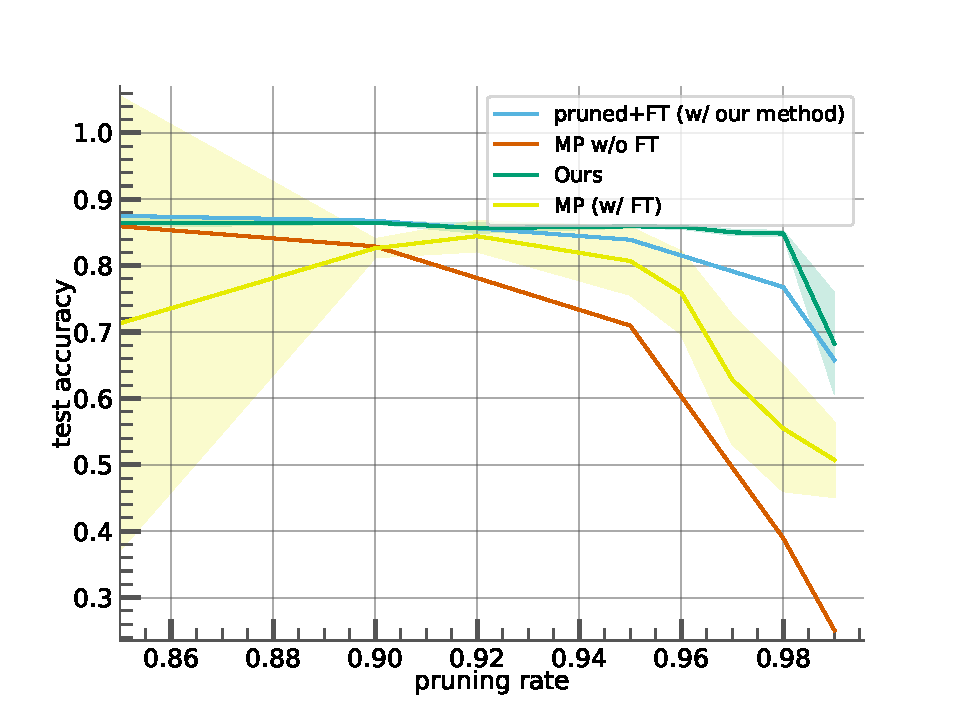
\includegraphics[width=0.49\textwidth]{chapter_1/assets/finetuning_cifar10_Conv4.pdf}}
  \subfloat[Conv4 CIFAR100\label{fig:chap1:finetuning_impact_conv4_cifar100}]{
  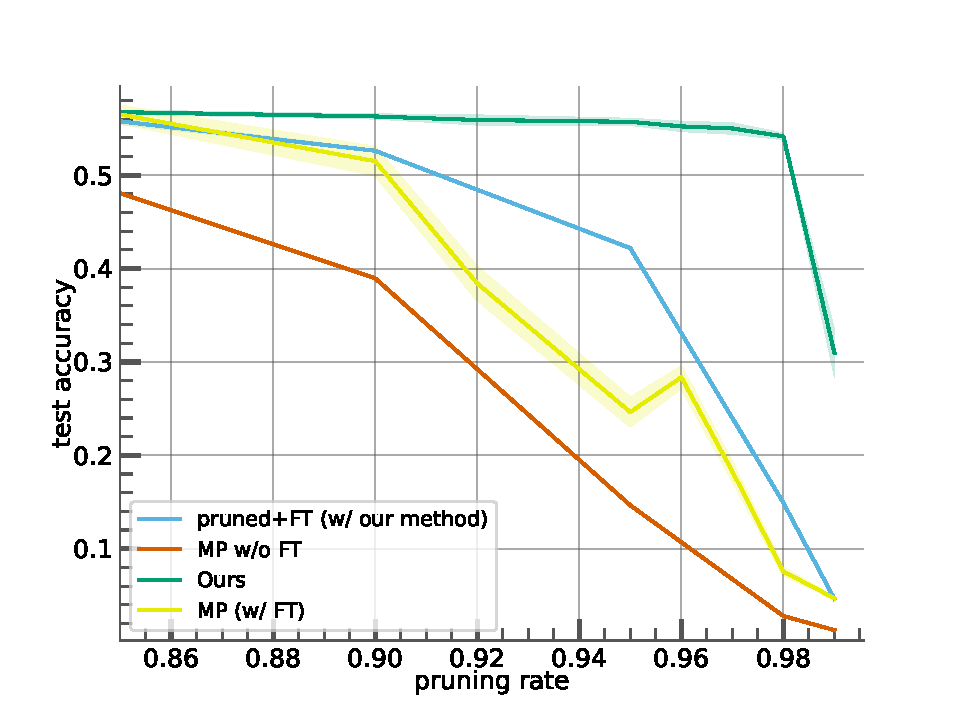
\includegraphics[width=0.49\textwidth]{chapter_1/assets/finetuning_cifar100_Conv4.pdf}}
  \caption{ Fine-tuning of a Conv4 network pruned by magnitude pruning
  (\emph{MP w/o FT}) on the CIFAR10 and CIFAR100 datasets for various pruning
  rates. Conventional (\emph{MP w/ FT}) fine-tuning is compared to fine-tuning
  with our method (\emph{pruned+FT (w/ our method)}). Our method is shown for
  comparison purposes (\emph{Ours}). On this network, our method performs better
  than other approaches. Fine-tuning the network with our method provides better
  results than fine-tuning it with a conventional method.}
    \label{fig:chap1:finetuning_impact_conv4}
\end{figure}


\begin{figure}
\centering
\subfloat[ResNet20 CIFAR10\label{fig:chap1:finetuning_impact_resnet20_cifar10}]{
  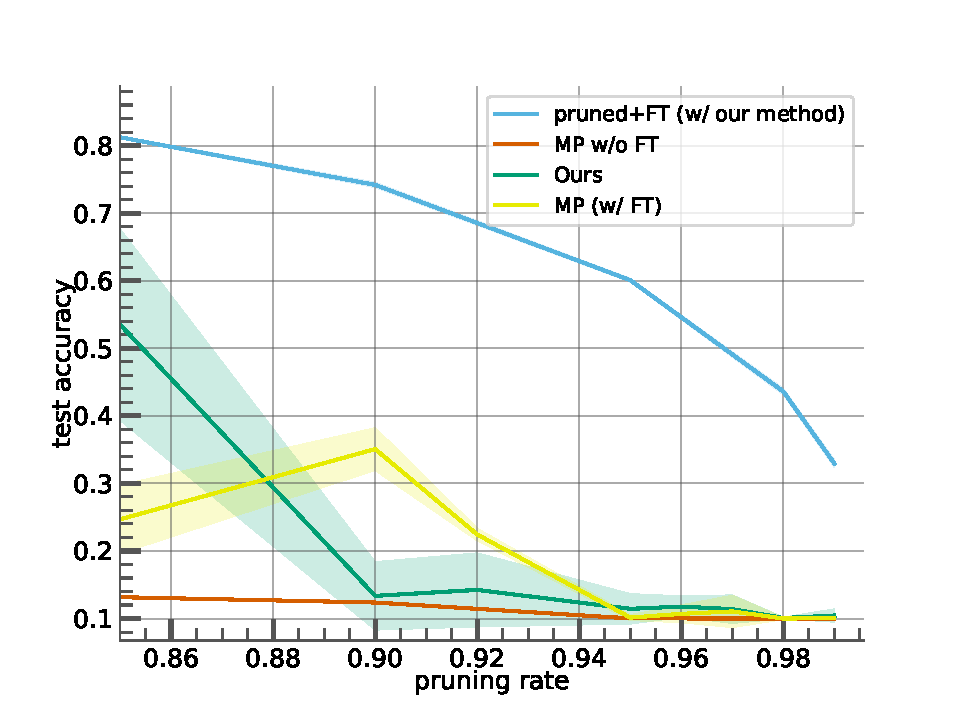
\includegraphics[width=0.49\textwidth]{chapter_1/assets/finetuning_cifar10_PrunableResNet20.pdf}}
  \subfloat[ResNet20 CIFAR100\label{fig:chap1:finetuning_impact_resnet20_cifar100}]{
  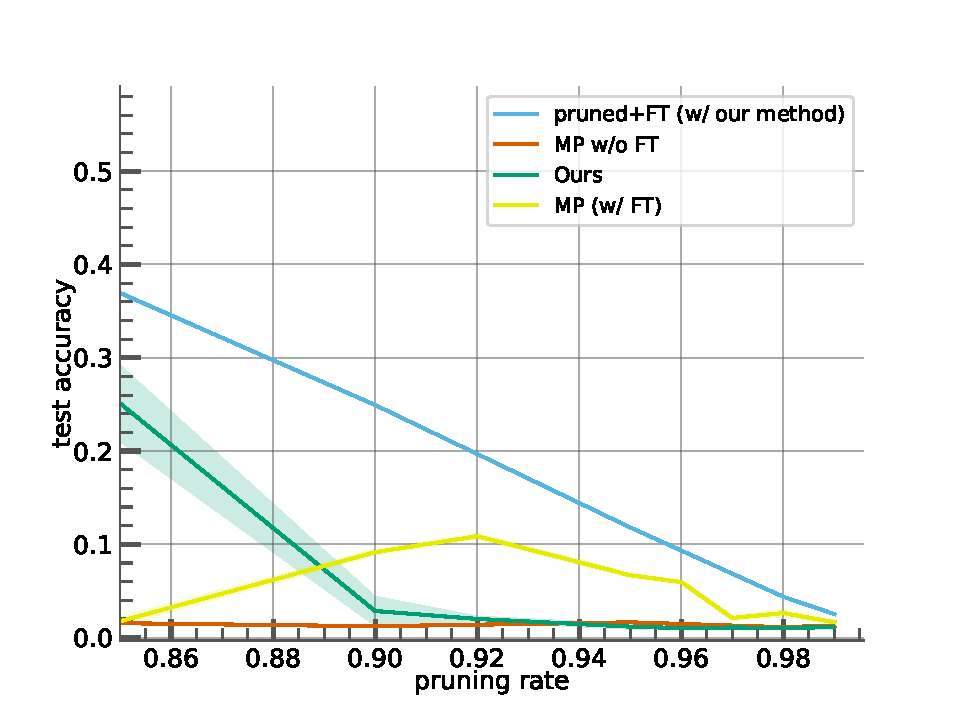
\includegraphics[width=0.49\textwidth]{chapter_1/assets/finetuning_cifar100_PrunableResNet20.pdf}}
  \caption{ Fine-tuning of a ResNet20 network pruned by magnitude
  pruning (\emph{MP w/o FT}) on the CIFAR10 and CIFAR100 datasets with various
  pruning rates. r  Conventional (\emph{MP w/ FT}) fine-tuning is compared to
  fine-tuning with our method (\emph{pruned+FT (w/ our method)}). Our method is
  shown for comparison purposes (\emph{Ours}). On this network, fine-tuning with
  our method considerably overperforms other approaches.}
    \label{fig:chap1:finetuning_impact_resnet20}
\end{figure}


\begin{figure}
\centering
\subfloat[VGG16 CIFAR10\label{fig:chap1:finetuning_impact_vgg16_cifar10}]{
  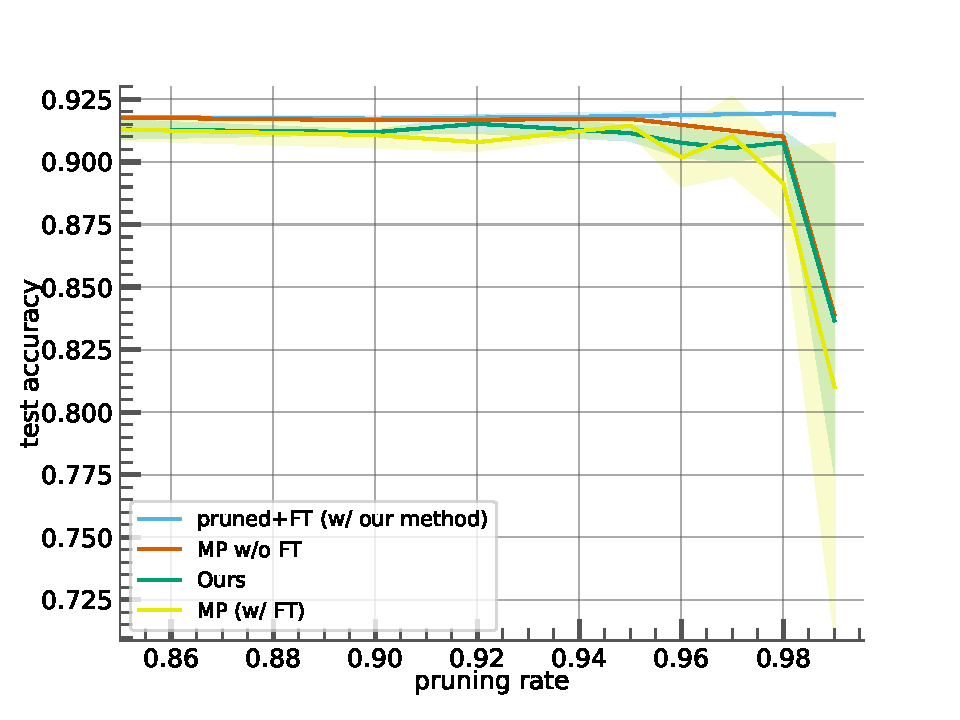
\includegraphics[width=0.49\textwidth]{chapter_1/assets/finetuning_cifar10_PrunableVGG16.pdf}}
  \subfloat[VGG16 CIFAR100\label{fig:chap1:finetuning_impact_vgg16_cifar100}]{
  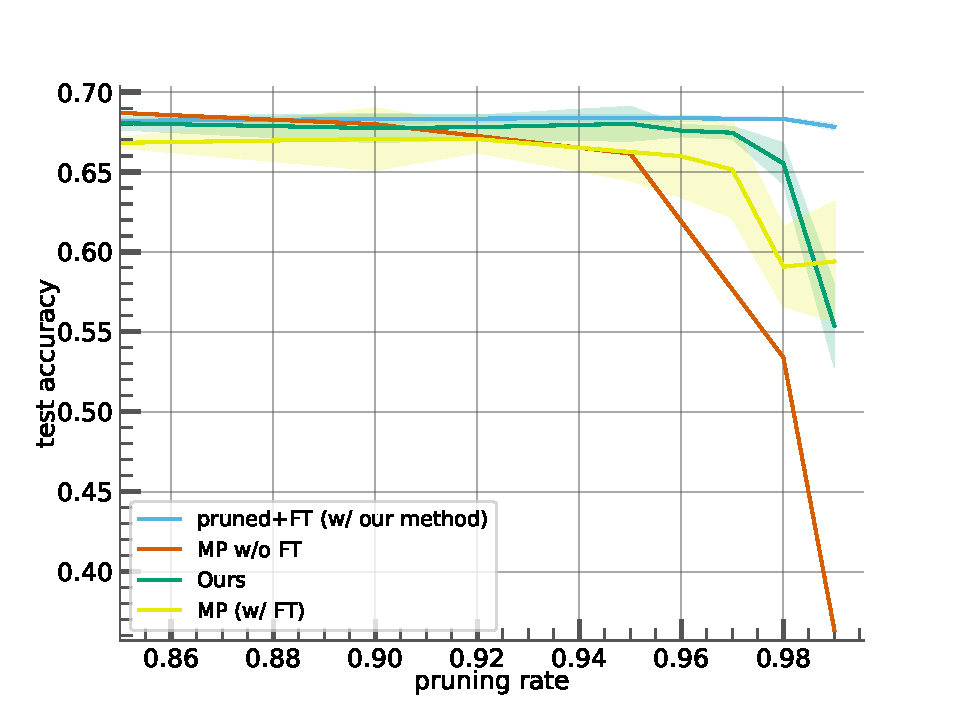
\includegraphics[width=0.49\textwidth]{chapter_1/assets/finetuning_cifar100_PrunableVGG16.pdf}}
  \caption{ Fine-tuning of a ResNet20 network pruned by magnitude
  pruning (\emph{MP w/o FT}) on the CIFAR10 and CIFAR100 datasets with various
  pruning rates. r  Conventional (\emph{MP w/ FT}) fine-tuning is compared to
  fine-tuning with our method (\emph{pruned+FT (w/ our method)}). Our method is
  shown for comparison purposes (\emph{Ours}). On this network, fine-tuning with
  our method performs on par with other methods up to 95\% of pruning. For
  higher pruning rates, it other performs other approaches.}
    \label{fig:chap1:finetuning_impact_vgg6}
\end{figure}

% endregion: fine-tuning




\section{Conclusion and Perspectives}
